Global PDF fits consist in a QCD analysis of hard-scattering measurements, 
possibly from a variety of different observables.
%
Parton distributions are parametrized at an initial energy scale, 
evolved up to the scale of the data via DGLAP 
equations~\eqref{eq:dglapunp}-\eqref{eq:dglappol}, and used to build up the 
theoretical predictions for the relevant observables.
%
In the corresponding factorization formul\ae, the factorization scale, $\mu$,
is usually set equal to the characteristic scale of the process, $Q$.
%
The best-fit parameters are then determined by minimization of a proper figure
of merit, such as the $\chi^2$.
%
In this section, we present the general global PDF fitting framework.
%
We discuss how PDFs are determined from hard-scattering observables,
paying attention to the assessment of PDF uncertainties.
%
We highlight the theory and the data used to fit both unpolarized and 
polarized PDFs and present a brief review of their state-of-the-art 
determination.

\subsubsection{General framework}
\label{sec:genframework}

\paragraph*{Fitting PDFs from hard-scattering data.} 
Parton distributions appear in the factorization formul{\ae} of a class of 
sufficiently inclusive processes, among which deep-inelastic scattering (DIS) 
and proton-(anti)proton collisions.
%
The factorization formul{\ae} for the unpolarized and polarized structure 
functions $F_1$ and $g_1$ were introduced in Eqs.~\eqref{eq:Fi}-\eqref{pdf}.
%
For the hadroproduction of a generic final-state $X$ in unpolarized 
(double polarized) proton-proton ($\overrightarrow{p}\overrightarrow{p}$) 
collisions, the corresponding factorized expressions read
\begin{align}
\sigma_{pp\to X}(s,\mu_F,\mu_R)=&\sum_{a,b}\int {\rm d}x_1 {\rm d}x_2\, 
f_a(x_1,\mu_F^2)f_b(x_2,\mu_F^2)\,
\hat{\sigma}_{ab\to X}(x_1,x_2,s;\mu_{F},\mu_R)\;,
\label{eq:LHCxsecunp}
\\
\Delta\sigma_{\overrightarrow{p}\overrightarrow{p}\to X}(s,\mu_F,\mu_R)=&\sum_{a,b}\int {\rm d}x_1 {\rm d}x_2\, 
\Delta f_a(x_1,\mu_F^2)\Delta f_b(x_2,\mu_F^2)\,
\Delta\hat{\sigma}_{ab\to X}(x_1,x_2,s;\mu_{F},\mu_R)\;,
\label{eq:LHCxsecpol}
\end{align}
where the unpolarized (polarized) hard cross-section 
$\hat{\sigma}_{ab\to X}$ ($\Delta\hat{\sigma}_{ab\to X}$) can be calculated 
perturbatively as an expansion in the QCD and electroweak (EW) 
running couplings.
%
The specific values of the momentum fractions
$x_i$ are related to the kinematics of the final state.
%
In particular, at LO it can be shown that
\be
x_{1,2}=\frac{M_X}{\sqrt{s}}e^{\pm y_X} \, ,
\ee
where $M_X$ and $y_X$ are the invariant mass and rapidity of the produced 
system and $\sqrt{s}$ is the center-of-mass energy.
%
The factorization and renormalization scales, $\mu_F$ and $\mu_R$, are 
usually taken equal to the hard scale of the process, $\mu_F=\mu_R=\mu=Q$.

When performing a global fit, the DGLAP evolution equations of the PDFs, 
Eqs.~\eqref{eq:dglapunp}-\eqref{eq:dglappol}, allow the PDF parametrization 
at one arbitrary input scale, typically $Q_0\sim 1$ GeV, to be connected to 
any other higher scale relevant for comparisons with the data.
%
The input PDF parameterization is usually chosen as
\begin{equation}
\label{eq:pdffunc}
f(x,Q_0,\{a_i\})= x^{a_1}(1-x)^{a_2}\:C(x,\{a_j\})\, ,
\end{equation}
where the parameters $\{a_i\}$ determine the PDF shape
and are different for each PDF flavor combination probed by the data.
%
The $(1-x)^{a_2}$ term, with $a_{2}>0$, ensures that the PDFs vanish in the 
elastic limit $x\to 1$. 
%
Specific values of the exponent $a_2$ are predicted by counting 
rules~\cite{Brodsky:1973kr}, although they are not always clearly
supported by phenomenological fits~\cite{Ball:2016spl,Nocera:2014uea}, 
in which they are therefore not used.
%
The $x^{a_1}$ term governs the low-$x$ PDF behavior. 
%
It is expected from considerations based on Regge theory, 
which also provides the values of the exponents $a_1$.
%
However, as for $a_2$, the value of $a_1$ is left free in the global fits..
%
The interpolating function $C(x)$ in Eq.~(\ref{eq:pdffunc})
affects the behavior of the PDFs away from the $x\to 0$ and $x\to 1$
extrapolation regions.
%
This is assumed to be a smoothly varying function of $x$, for which a variety 
of parametrizations can be made (see below).
%
The charm and bottom heavy quark PDFs $c(x,\mu)$ and $b(x,\mu)$ are usually not
parametrized as in  Eq.~(\ref{eq:pdffunc}) but rather
generated by perturbative emission of gluons and light quarks.
%
The possibility of parametrizing and fitting the charm PDF
on the same footing as light quark PDFs has been recently 
explored~\cite{Ball:2016neh}.

Some form for the interpolating function $C(x)$ in Eq.~\eqref{eq:pdffunc} 
must be assumed.
%
The simplest ansatz, which has been very widely used, is to take a basic 
polynomial form in $x$ (or $\sqrt{x}$), such as
\begin{equation}\label{eq:lpower}
C(x)=1+a_2\sqrt{x}+a_3 x+...\;.
\end{equation}
Functional forms of this type are, for example, taken in CJ, HERAPDF and 
earlier MMHT and CT sets (see below for the references to each set). 
%
More recently, the CT and MMHT collaborations expand 
in terms of a basis of  Bernstein and Chebyshev polynomials, respectively.
%
While formally equivalent to the simple polynomial expansion
Eq.~\eqref{eq:lpower}, these are much more convenient for fitting as the 
number of free parameters $n_{\rm par}$ is usually increased.
%
In the latest CT and MMHT sets, there are between 20 and 40 free parameters in 
total, though some of these are kept fixed when evaluating the
Hessian PDF uncertainties to control for redundancy between the parameters.
%
Furthermore, the use of orthogonal polynomials, like Bernstein or Chebyshev 
polynomials, allows one to decouple the parameters in $C(x)$ and to uniformly
sample its possible functional shapes.

An alternative approach to the PDF parametrization Eq.~\eqref{eq:lpower}
is adopted by the NNPDF collaboration. 
%
Here, the interpolating function $C(x)$ is modelled with 
a multi-layer feed forward neural network.
%
In practice, this allows for a greatly increased number of free parameters, 
typically an order of magnitude higher than other sets.
%
The form of Eq.~\eqref{eq:pdffunc} is still assumed, but
now $C(x)={\rm NN}(x)$ is parametrized as a neural network.
%
The $x^{a_1}(1-x)^{a_2}$ term that multiplies the NN represents
a preprocessing factor that speeds up the minimization procedure
and that is determined via an iterative procedure.
%
Because of the redundancy of the parametrization, the statistical noise in 
the data could be learned in the minimization procedure.
%
In order to avoid such a drawback, the data are split into validation and 
training sets, then the best-fit is determined by
cross-validation~\cite{Forte:2002fg,DelDebbio:2004xtd}.
%
A similar technique is used also in the JAM 
fits~\cite{Sato:2016tuz,Ethier:2017zbq}.

Once the PDF parametrization is chosen, the best-fit PDF parameters
and their uncertainty should be determined via a fitting methodology
which minimizes a suitable statistical estimator, typically the $\chi^2$.
%
There exist different alternative definitions of the $\chi^2$
to be used in the global fits~\cite{Ball:2012wy}. 
%
For instance one frequently used definition is
\begin{equation}
\chi^2 
= 
\sum_{i,j}^{N_{\rm dat}} (T_i(\{a_k\}) - D_i) 
({\rm cov^{-1}})_{ij} (T_j(\{a_k\}) - D_j)\,,
\label{eq:chi2}
\end{equation}
where $N_{\rm dat}$ is the number of data points of a given experiment,
$T_i$ and $D_i$ are the corresponding theoretical predictions
and experimental data, and $({\rm cov^{-1}})_{ij}$ is the inverse of the 
experimental covariance matrix.
%
The theoretical predictions $T_i(\{a_k\})$ depend on the input set of 
parameters $\{a_k\}$ via the PDF parametrization, see Eq.~\eqref{eq:pdffunc}.
%
Therefore, Eq.~\eqref{eq:chi2} assesses the agreement between theory and data.

The covariance matrix $({\rm cov})_{ij}$ accounts for the various sources of 
experimental systematic uncertainties and also allows for several
different definitions.
%
One example is the so-called $t_{0}$ prescription~\cite{Ball:2009qv}, 
where a fixed theory prediction $T_{i}^{(0)}$ is used to define the  
contribution to the $\chi^2$ from the multiplicative systematic uncertainties, 
namely
\be
\label{eq:covmat_t00}
({\rm cov})_{ij}=
\delta_{ij} \sigma_{\rm stat}^2 + 
\sum_{\alpha=1}^{N_c}\sigma^{(c)}_{i,\alpha}\sigma^{(c)}_{j,\alpha}D_{i} D_{j}
+ \sum_{\beta=1}^{N_{\cal L}} \sigma_{i,\beta}^{({\cal L})}\sigma_{j,\beta}^{({\cal L})}
T^{(0)}_{i} T^{(0)}_{j}\, .
\ee
Here $\sigma_{\rm stat}$ is the uncorrelated uncertainty,
and $\sigma^{(c)}_{i,\alpha}$ ($\sigma^{(\cal L)}_{i,\beta}$) are the various sources 
of additive (multiplicative) systematic uncertainties.
%
The $t_0$ prescription is needed to avoid the D'Agostini 
bias~\cite{DAgostini:2003syq,DAgostini:1993arp}, a downwards
bias of the statistical estimators for the central value and the uncertainty
of the theoretical predictions due to the rescaling induced by  multiplicative 
uncertainties.
%
See~\cite{Ball:2009qv} and references therein for details and the alternative
{\it penalty-trick} prescription.

\paragraph{PDF uncertainties.}
Determining the best-fit values of the PDF parameters is not enough: one also 
needs to estimate the associated PDF uncertainties, possibly separated into 
the various sources of experimental, methodological and theoretical 
uncertainties.
%
In this respect, there are two main methods to determine PDF uncertainties, the 
{\it Hessian} and the {\it Monte Carlo} methods.\footnote{The Lagrange 
multiplier method~\cite{Stump:2001gu} is also frequently used for dedicated 
studies of PDF uncertainties.}

The Hessian method~\cite{Pumplin:2001ct} is based on the parabolic
expansion of the $\chi^2$ in the vicinity of its minimum 
\be
\label{eq:hessianexpansion}
\Delta\chi^2 \equiv \chi^2- \chi^2_{\rm min}
=\sum_{i,j=1}^{n_{\rm par}}H_{ij}\lp a_i-a_i^0\rp
\lp a_j-a_j^0\rp \, ,
\ee
where the $n_{\rm par}$ PDF fit parameters are denoted by 
$\{a_1,\ldots,a_{n_{\rm par}}\}$, the best-fit values that minimize the
$\chi^2$ are indicated by $\{a_1^0,\ldots,a^0_{n_{\rm par}}\}$,
and the Hessian matrix is defined as
\be
H_{ij}\equiv \frac{1}{2} \frac{\partial^2\chi^2}{\partial a_i
\partial a_j}\Bigg|_{\{\vec{a}\}=
\{\vec{a}^0\}}\, .
\ee
By diagonalizing this Hessian matrix, it becomes possible
to represent PDF uncertainties in terms of orthogonal eigenvectors
within a fixed tolerance $T=\sqrt{\Delta\chi^2}$.
%
These eigenvectors can then be used to estimate the PDF uncertainty for 
arbitrary cross-sections, using the master formula of Hessian PDF sets for 
the uncertainty of the cross-section $\mathcal{F}$, namely
\be
\label{eq:hessianmaster2}
\sigma_{\mathcal{F}}=\frac{1}{2}\lp \sum_{i,j}^{n_{\rm par}}
\lc \mathcal{F}(S_i^+)-\mathcal{F}(S_i^-) \rc^2 \rp^{1/2} \, ,
\ee
where $S_i^{\pm}$ correspond to the $i$-th eigenvector
associated to positive and negative variations with respect
to the best fit value.

The Monte Carlo method~\cite{Forte:2002fg,DelDebbio:2004xtd} is based 
on constructing a representation of the probability distribution of the 
experimental data in terms of a large number $N_{\rm rep}$ of {replicas},  
which encode all the information on central values, variances and 
correlations provided by the experiments.
%
Specifically, given an experimental measurement of a hard-scattering
observable $F_{I}^{\rm (exp)}$, with total uncorrelated uncertainty 
$\sigma_{I}^{\rm (stat)}$, $N_{\rm sys}$ fully correlated systematic uncertainties 
$\sigma^{\rm (corr)}_{I,c}$ and $N_a$ ($N_r$) absolute (relative) normalization 
uncertainties $\sigma^{\rm (norm)}_{I,n}$, the Monte Carlo replicas are 
constructed using the expression
\be
\label{eq:replicas}
F_{I}^{(\art)(k)}
=
S_{I,N}^{(k)} F_{I}^{\rm (\mrexp)}\lp 1
+
\sum_{c=1}^{N_{\rm sys}}r_{I,c}^{(k)}\sigma^{\rm (corr)}_{I,c}
+
r_{I}^{(k)}\sigma_{I}^{\rm (stat)}\rp
\ , \quad k=1,\ldots,N_{\rep} \ ,
\ee
where $S_{I,N}^{(k)}$ is a normalization prefactor.
%
The variables $r_{I,c}^{(k)},r_{I}^{(k)},r_{p,n}^{(k)}$ are
univariate Gaussian random numbers.
%
For each individual replica, the random fluctuations associated to a given 
fully-correlated systematic uncertainty will be the same
for all data points, $r^{(k)}_{I,c}=r^{(k)}_{I',c}$.

Parton distribution fits are then performed separately on each of the 
Monte Carlo replicas.
%
The resulting ensemble of PDFs samples the probability density in the space
of PDFs.
%
The expectation function of a generic observable $ \mathcal{F} [ \{  f \}]$,
depending on the fitted set of PDFs $\{f\}$,
is evaluated as an average over the replica sample,
\be
\label{masterave}
\la \mathcal{F} [ \{  f \}] \ra
= \frac{1}{N_{\rm rep}} \sum_{k=1}^{N_{\rm rep}}
\mathcal{F} [ \{  f^{(k)} \}] \, .
\ee
The corresponding uncertainty is determined as the variance of the
Monte Carlo sample,
\be
\sigma_{\mathcal{F}} =
\left( \frac{1}{N_{\rm rep}-1}
\sum_{k=1}^{N_{\rm rep}}   
\lp \mathcal{F} [ \{  f^{(k)} \}] 
-   \la \mathcal{F} [ \{  f \}] \ra\rp^2 
 \right)^{1/2}.
\label{mastersig}
\ee
Likewise, other properties of the underlying PDF probability distribution, 
such as skewness and kurtosis, could be readily computed.

%In the following sections, when comparing the results of global PDF fits
%with the results of lattice QCD calculations we will use 
%Eqs.~(\ref{eq:hessianmaster2}) and~(\ref{mastersig}) to evaluate the PDF 
%uncertainties of Hessian and Monte Carlo PDF sets.
%%
%Unless otherwise stated, the quoted PDF uncertainties correspond to 
%the 68\%-CL intervals.

Given a PDF set in the Hessian representation, it is possible to construct
the corresponding Monte Carlo representation~\cite{Watt:2012tq,Hou:2016sho}
and vice-versa~\cite{Gao:2013bia,Carrazza:2015aoa}.

There are additional sources of theoretical uncertainty that are not accounted 
for, either in the Hessian or in the MC methods.
%
The first one is the parametric uncertainty due to finite uncertainties 
associated to the input values of the physical parameters used in the global 
fit, such as $\alpha_s(m_Z)$ and the charm mass $m_c(m_c)$.
%
These additional uncertainties can be included by repeating the fits for 
different values of the physical parameters and then suitably combining 
the results.
%
The second source of theoretical uncertainty neglected in PDF fits
is that due to the truncation of the perturbative expansion, known
as missing higher-order uncertainty (MHOU).
%
While this is expected to be small for NNLO fits, currently its size is unknown.

%Extend here the discussion along the lines suggested by Alberto?

\subsubsection{Unpolarized PDFs}
\label{sec:unpPDFs}

\paragraph*{Theoretical features.}
While the general $x$ dependence of the PDFs is determined by
nonperturbative QCD dynamics, there are still a number
of theoretical constraints that any PDF set should satisfy. 
%
These should be imposed during the fit procedure.

First, since the proton has the quantum numbers of two up quarks and one 
down quark, the following quark number sum rules, given in terms of zeroth
moments, must be satisfied: 
\begin{eqnarray}
\int_{0}^{1}dx\ \left[u(x,\mu)-\bar{u}(x,\mu)\right] 
& =\left\langle 1\right\rangle _{u^{-}}= & 2 \, ,\nonumber \\
\int_{0}^{1}dx\ \left[d(x,\mu)-\bar{d}(x,\mu)\right] 
& =\left\langle 1\right\rangle _{d^{-}}= & 1 \, ,
\label{eq:valencesumrules}\\
\int_{0}^{1}dx\ \left[s(x,\mu)-\bar{s}(x,\mu)\right] 
& =\left\langle 1\right\rangle _{s^{-}}= & 0 \, .\nonumber
\end{eqnarray}
%
Similar constraints hold for heavy quarks: 
$\left\langle 1\right\rangle _{c^{-}}=\left\langle 1\right\rangle _{b^{-}}
=\left\langle 1\right\rangle _{t^{-}}=0$.
%
The valence sum rules, Eqs.~\eqref{eq:valencesumrules}, should be satisfied at 
any scale $\mu$. 
%
Indeed it can be shown that if they hold at the input parametrization scale 
$\mu=Q_0$, they are subsequently respected by DGLAP evolution.
%
Therefore, for these distributions we must have $a_1>-1$ in
Eq.~(\ref{eq:pdffunc}), otherwise Eqs.\eqref{eq:valencesumrules} 
would be ill-defined.

Second, PDFs should satisfy the conservation of energy-momentum derived from
the QCD Lagrangian.
%
In other words, the proton's total momentum should be equal 
to the sum of the momentum carried by all its constituents
(the so-called momentum sum rule):
\begin{equation}
\label{eq:mom}
1 
= 
\left\langle x\right\rangle _{g}
+
\left\langle x\right\rangle _{u^{+}}
+
\left\langle x\right\rangle _{d^{+}}
+
\left\langle x\right\rangle _{s^{+}}
+
\left\langle x\right\rangle _{c^{+}}
+
\left\langle x\right\rangle _{b^{+}}
+
\left\langle x\right\rangle _{t^{+}}+\ldots\,,
\end{equation}
%
where the ellipsis represents any other partonic components (such
as a photon). 
%
The first moments, $\left\langle x\right\rangle _{f}$, are defined in analogy 
to Eqs.~\eqref{eq:umoment1}-\eqref{eq:uplusmoment1}. 
%
In order to avoid a divergent contribution, we must have $a_1>-2$ in 
Eq.~\eqref{eq:pdffunc} for the non-valence distributions.
%
Typically it turns out that $-2<a_1<-1$ for such distributions, hence 
the number of soft partons grows very quickly at small $x$, although the 
momentum fraction carried by them is well-defined and finite.
%
As in the case of the valence sum rules, the momentum
sum rule is preserved by the DGLAP evolution equations.

Theoretical calculations of DIS and hadronic cross-sections at the highest 
perturbative order available should be used.
%
Currently, this implies using NNLO for the QCD corrections and NLO
for the EW and photon-induced effects~\cite{Manohar:2016nzj,Manohar:2017eqh}.
%
Thanks to recent progress in higher-order calculations, these results
are available for most of the processes entering the global
PDF fits~\cite{Currie:2016bfm,Campbell:2016lzl,Czakon:2016dgf,
Boughezal:2017nla,Li:2012wna}, including differential distributions with 
colored particles in the final state.

These calculations should be provided in
a format such that the evaluation of the hadronic
cross-sections, Eq.~\eqref{eq:LHCxsecunp}, is not too burdensome
from a computational point of view.
%
To bypass the limitations of the lengthy (N)NLO
computations, a number of fast interfaces have
been developed that allow for the efficient calculation
of NLO (and NNLO) fully differential hadronic cross-sections,
among which {\tt APPLgrid}~\cite{Carli:2010rw},
{\tt FastNLO}~\cite{Wobisch:2011ij} and {\tt aMCfast}~\cite{Bertone:2014zva}.

\paragraph*{Experimental data.}
A broad set of input hard-scattering cross-sections from DIS and
proton-(anti)proton collisions, providing information on the PDFs over a wide 
range of $x$ and for different flavor combinations, is used in modern PDF fits.
%
Inclusive DIS measurements have been realized with electron, muon and neutrino
(and the corresponding antiparticles) off protons, deuterons and
heavy nuclear targets. 
%
While traditional PDF fits were based mostly on DIS structure functions, 
and Drell-Yan and inclusive jet cross-sections, in recent years many other 
processes have proved important for constraining PDFs, among which
top-quark pair production~\cite{Czakon:2016olj}, the $p_T$ distribution of $Z$ 
bosons~\cite{Boughezal:2017nla} and $D$ meson production in 
the forward region~\cite{Gauld:2016kpd}.

In Fig.~\ref{fig:kinplot-report} we show the representative kinematic coverage 
in the $(x,Q^2)$ plane of the DIS and proton-(anti)proton hard-scattering 
measurements that are used as input in a typical global fit of unpolarized 
PDFs, in this case NNPDF3.1~\cite{Ball:2017nwa}.
%
In order to facilitate visualization, different datasets have been clustered 
together into families of related processes.
%
For hadronic cross-sections, LO kinematics is assumed to map
each experimental bin into a pair of points in the $(x,Q^2)$ plane.
%
The fact that similar regions in the $(x,Q^2)$ plane are covered by
different processes is essential to achieve quark
flavor separation and to constrain the gluon PDF.

Abundant precise data from SLAC and Jefferson Lab exist also in the 
bottom right corner of the $(x,Q^2)$ plane, where however power corrections 
need to be accounted for 
in QCD fits~\cite{Alekhin:2017kpj,Owens:2012bv,Accardi:2016qay}.
%
They are not shown in Fig.~\ref{fig:kinplot-report} because they are excluded 
from the NNDPF3.1 fit by the kinematic cut on the invariant mass of the final
state $W^2<12.5$ GeV$^2$ adopted there.

%-------------------------------------------------------------------------------
\begin{figure}[!t]
\centering
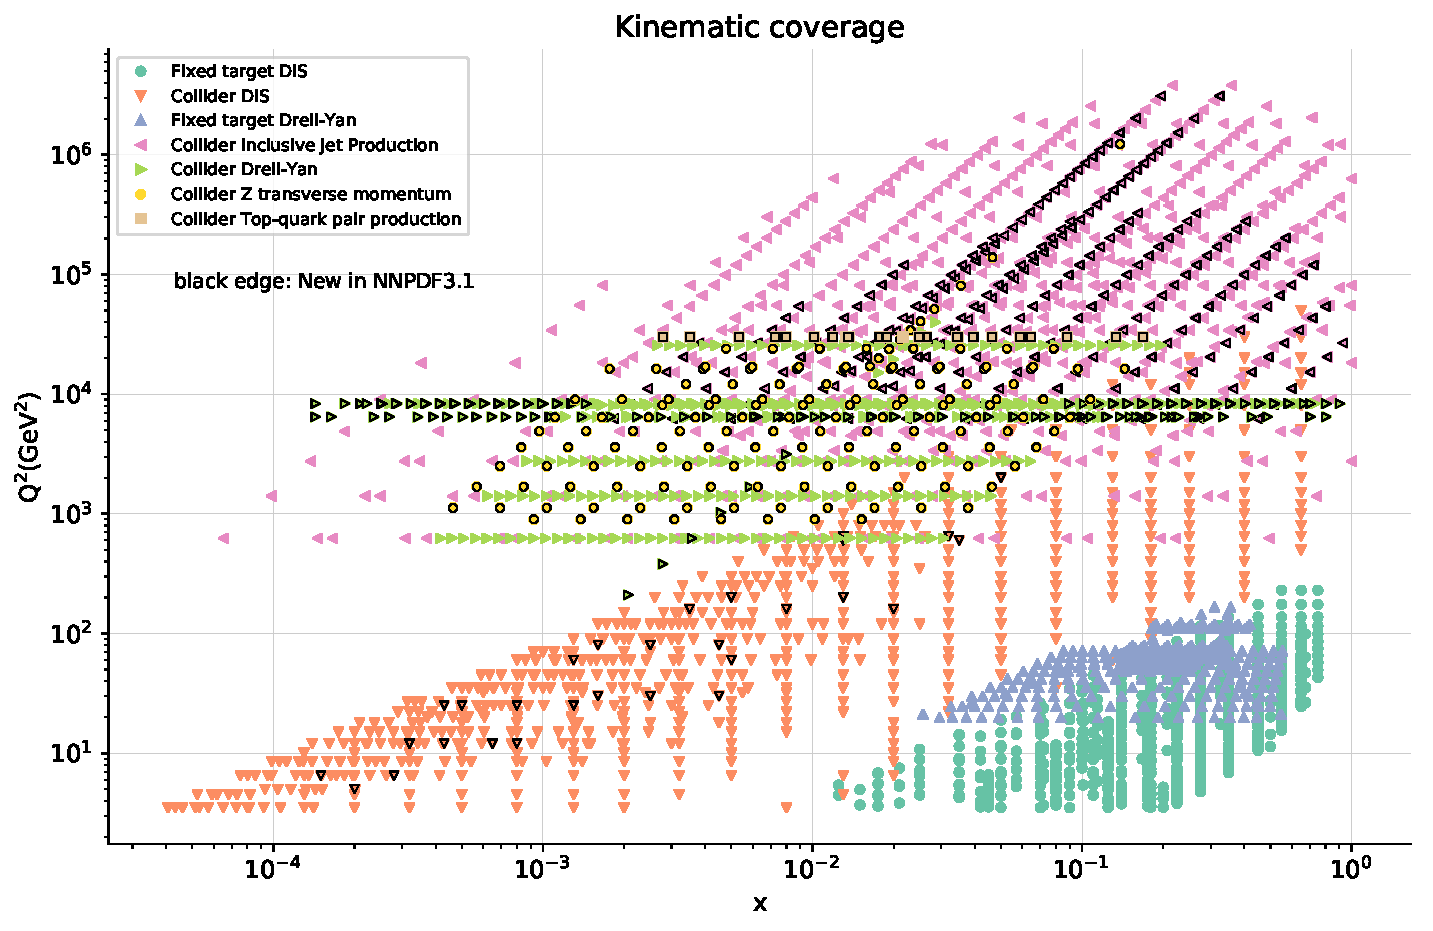
\includegraphics[scale=0.60]{plots/kinplot-report.pdf}
\caption{\small Representative kinematic coverage in the $(x,Q^2)$ plane
 of the DIS and proton-(anti)proton hard-scattering measurements that are
 used as input in a typical fit of unpolarized PDFs, 
 NNPDF3.1~\cite{Ball:2017nwa}.
 %
 Different datasets have been clustered together into families of
 related processes.
 %
 For hadronic cross-sections, leading order kinematics is assumed to map
 each experimental bin to a pair of points in the $(x,Q^2)$ plane.
 %
 Additional precise data from SLAC and Jefferson Lab exist also in the 
 bottom right corner of the $(x,Q^2)$ plane, although they were excluded from 
 the NNPDF3.1 fit by the cut on the invariant mass of the final 
 state $W^2<12.5$ GeV$^2$ adopted there.}
\label{fig:kinplot-report} 
\end{figure}
%-------------------------------------------------------------------------------

\paragraph*{State-of-the-art global PDF fits.}
%
Various collaborations provide regular updates of their global unpolarized
PDF fits.
%
The latest fits from the three main global fitting collaborations
are CT14~\cite{Dulat:2015mca}, MMHT14~\cite{Harland-Lang:2014zoa} and
NNPDF3.1~\cite{Ball:2017nwa}.
%
These fits are performed up to NNLO in the strong coupling (with central value
$\alpha_s(m_Z)=0.118$), and include data from the HERA $e^{\pm} p$ collider, 
fixed (nuclear and proton) target experiments, the Tevatron $p\overline{p}$ 
collider and the LHC. 
%
The ABMP16~\cite{Alekhin:2017kpj} set fits to a similar global data set
(although excluding jet production) but differs in its treatment of errors,
 heavy flavors and the low-$Q^2$ and large-$x$ regions.
%
The HERAPDF2.0~\cite{Abramowicz:2015mha} set fits to the final combined HERA 
Run I + II data set only, with the aim of determining the PDFs from a 
completely consistent DIS data sample; in $x$ regions that are less constrained 
by HERA data, the uncertainties can be quite large.
%
The CJ15~\cite{Accardi:2016qay} NLO set focuses on constraining the PDFs at 
higher $x$ by lowering $Q^2$ and $W^2$ cuts in DIS.
%
This greatly increases the available data, but requires additional modeling of 
power-like ${\cal O}(1/Q^2)$ corrections.

The features of each PDF set have ben discussed in detail in 
Refs.~\ref{Butterworth:2015oua,Accardi:2016ndt}, including the 
dataset, the fitting methodology, the theoretical details of the 
corresponding QCD analyses, and, most importantly, the uncertainties
coming from each of these aspects.

%A detailed discussion of the similarities and differences between
%PDF sets, which is beyond the scope of this document,
%can be found in the PDF4LHC report~\cite{Butterworth:2015oua}.
%%
%It suffices here to say that all PDF sets listed above use the Hessian
%method to determine PDF uncertainties,
%except NNPDF which is based on the Monte Carlo approach.

In Fig.~\ref{fig:globalfits}
we present a snapshot of the current understanding
of the proton structure in the global PDF fitting framework.
%
We compare the CT14, MMHT2014
and NNPDF3.1 NNLO PDF sets at $Q=100$ GeV, normalized
to the central value of the last.
%
From top to bottom and from left to right we show the
$u$, $\bar{d}$ and $s$ quark PDFs and the gluon PDF.
%
The error bands indicate the 68\%-confidence level (CL) PDF uncertainties
associated to each set, computed with the corresponding master formula.
%
We observe that differences for the up quark PDF
are small, at the few percent level, but greater differences
are observed for the sea quarks, in particular
in the medium and large-$x$ region.
%
For the gluon there is reasonable agreement except in the large-$x$ region, 
where NNPDF3.1 is softer than CT14 and MMHT14.
%
Any other comparison plots between PDFs can be straightforwardly
obtained using the {\tt APFEL-Web} online plotting 
interface~\cite{Carrazza:2014gfa}.

%-------------------------------------------------------------------------------
\begin{figure}[!t]
\centering
 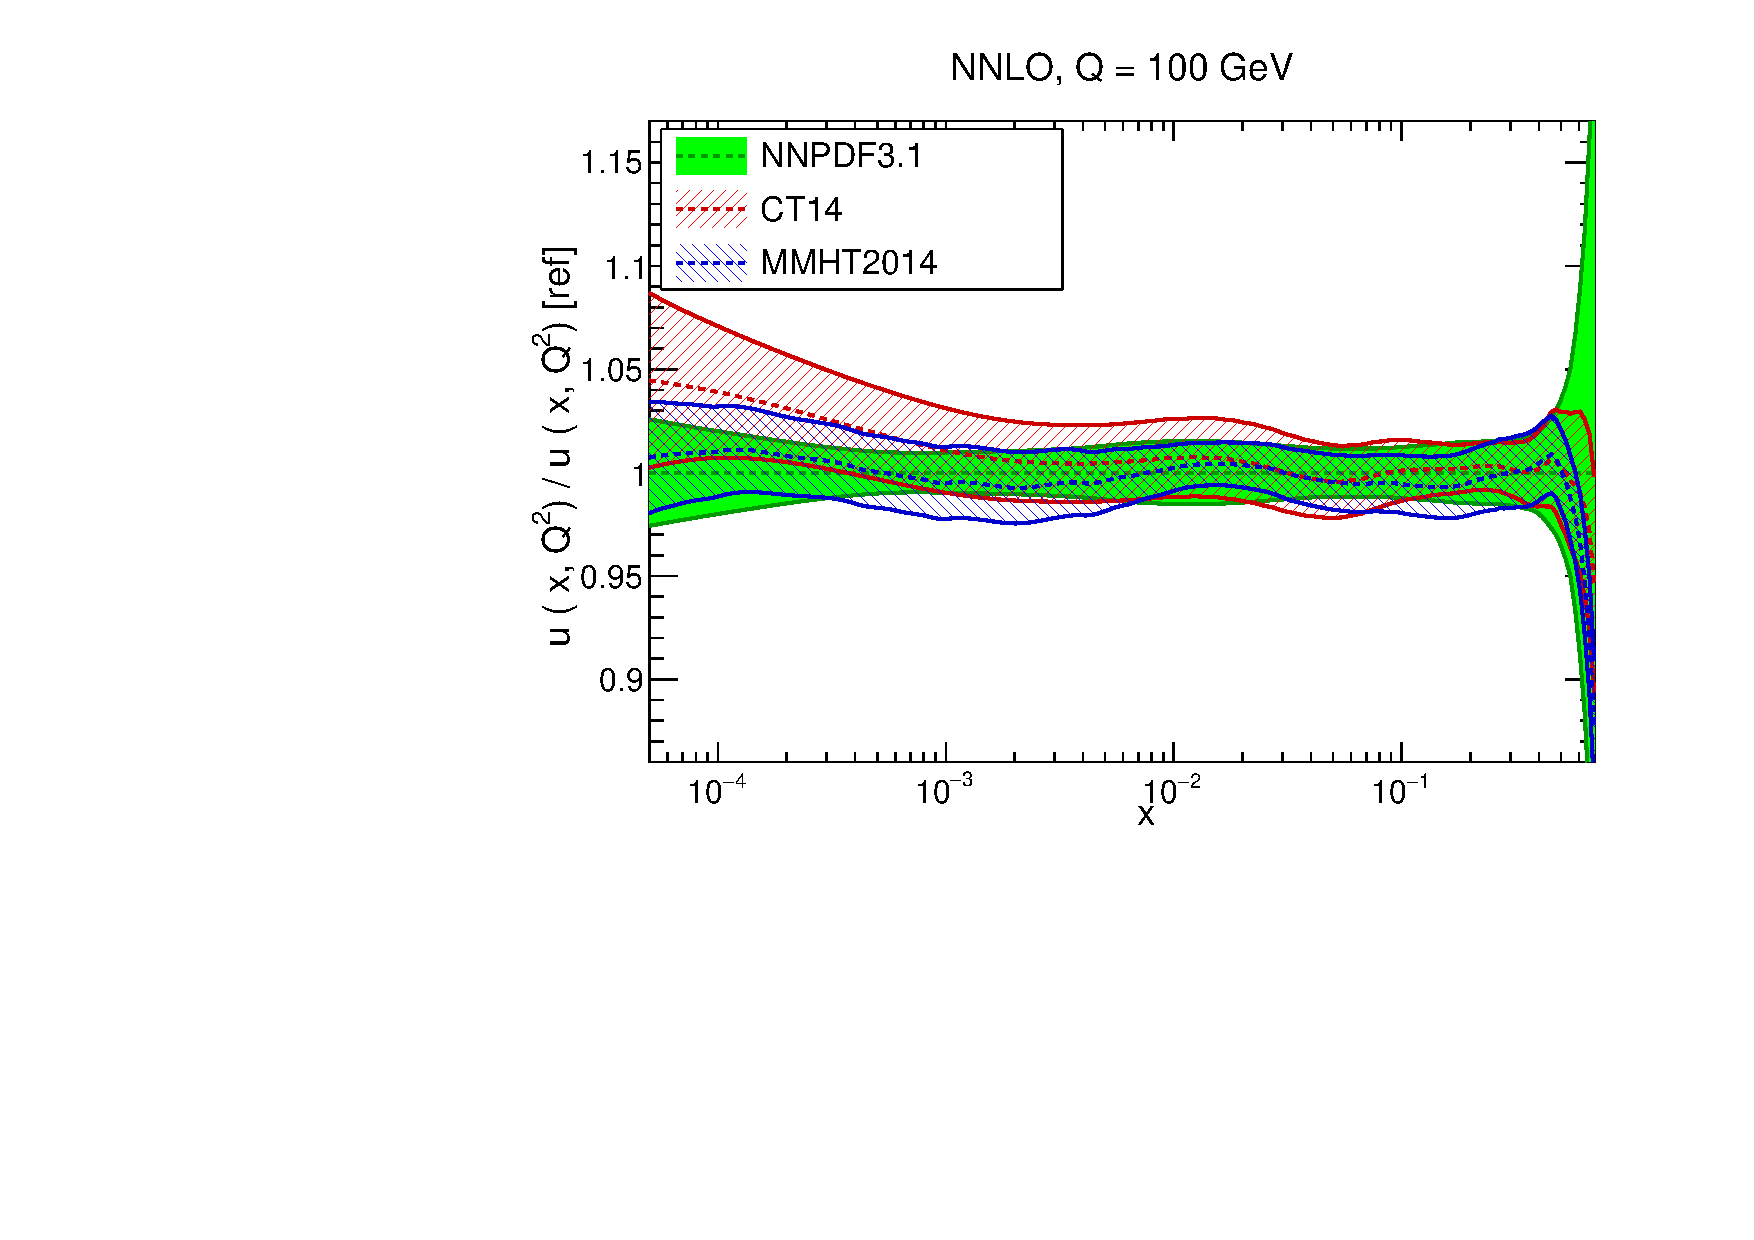
\includegraphics[scale=0.37]{plots/xu-31-nnlo-globalfits.pdf}
 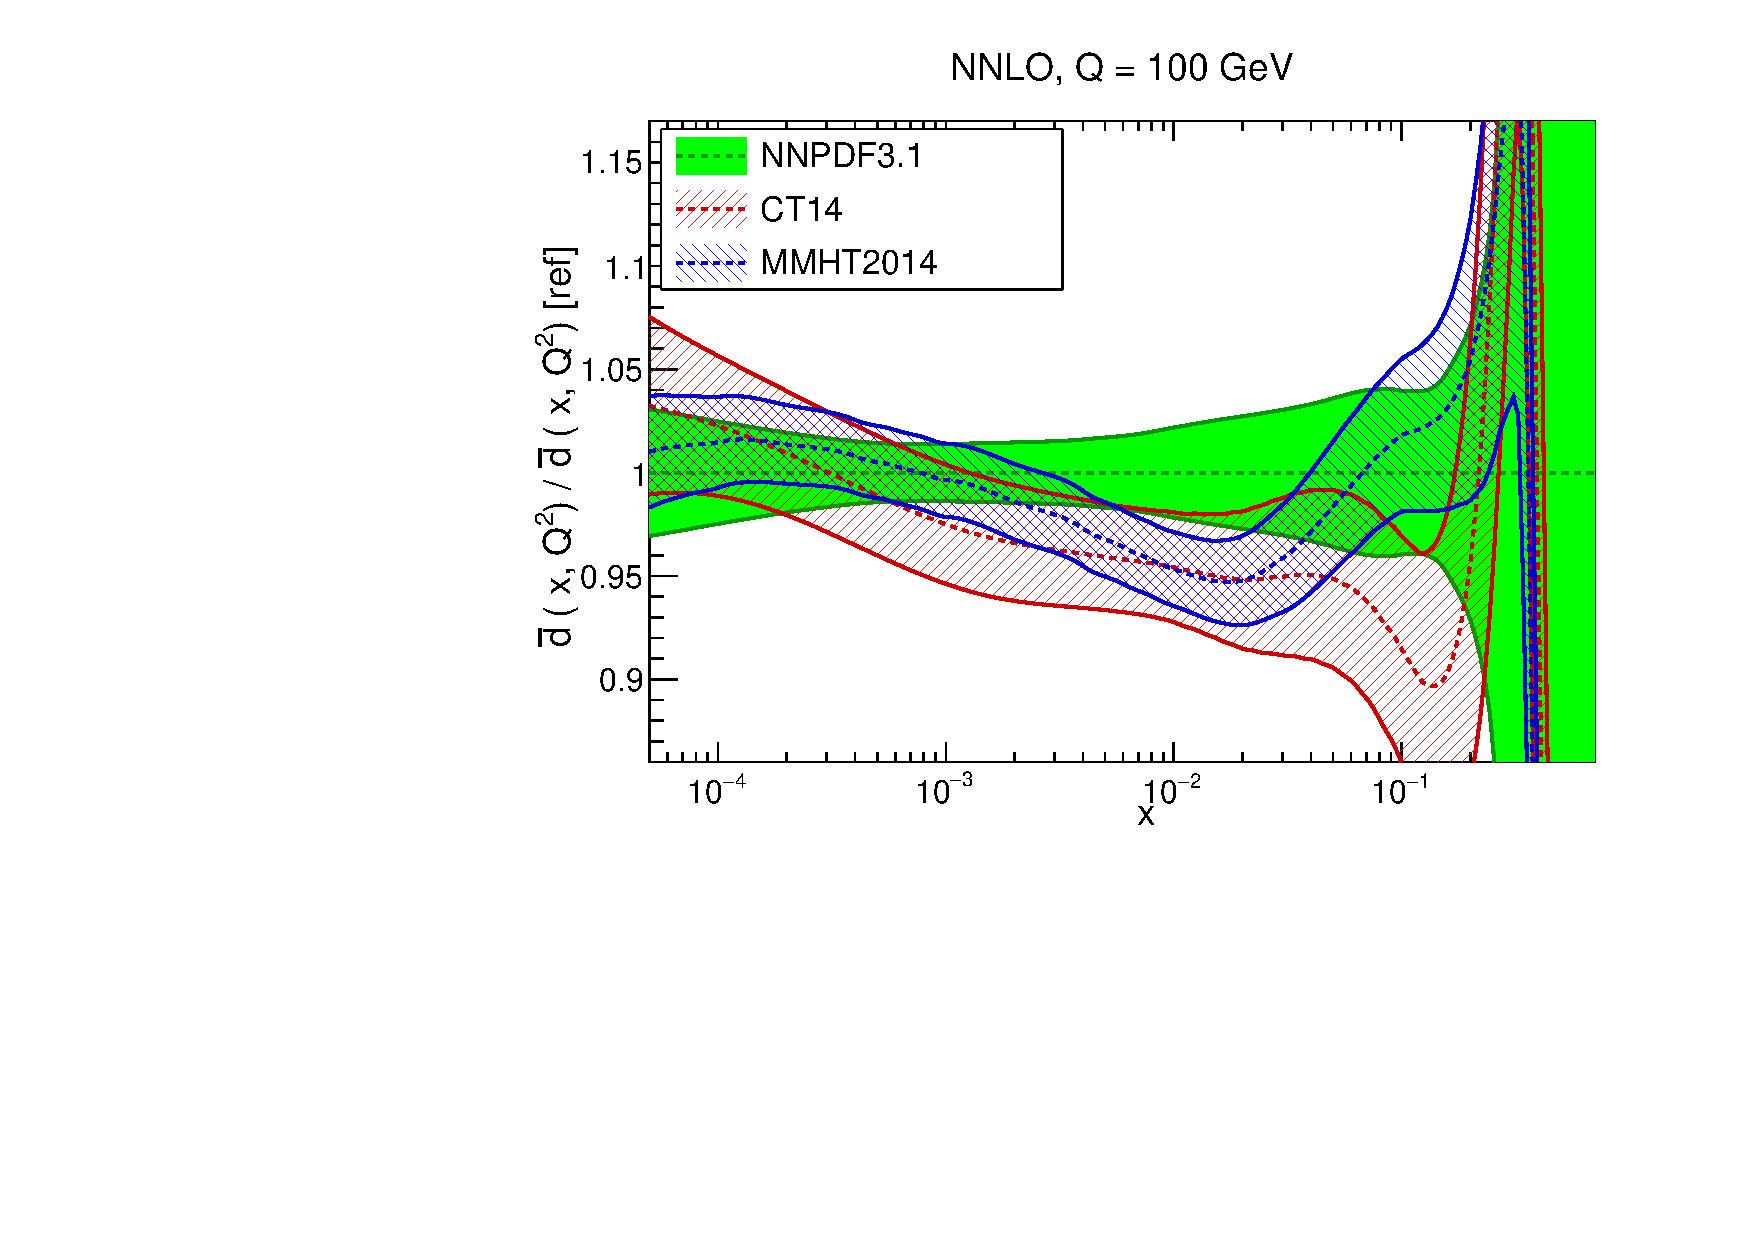
\includegraphics[scale=0.37]{plots/xdbar-31-nnlo-globalfits.pdf}\\
 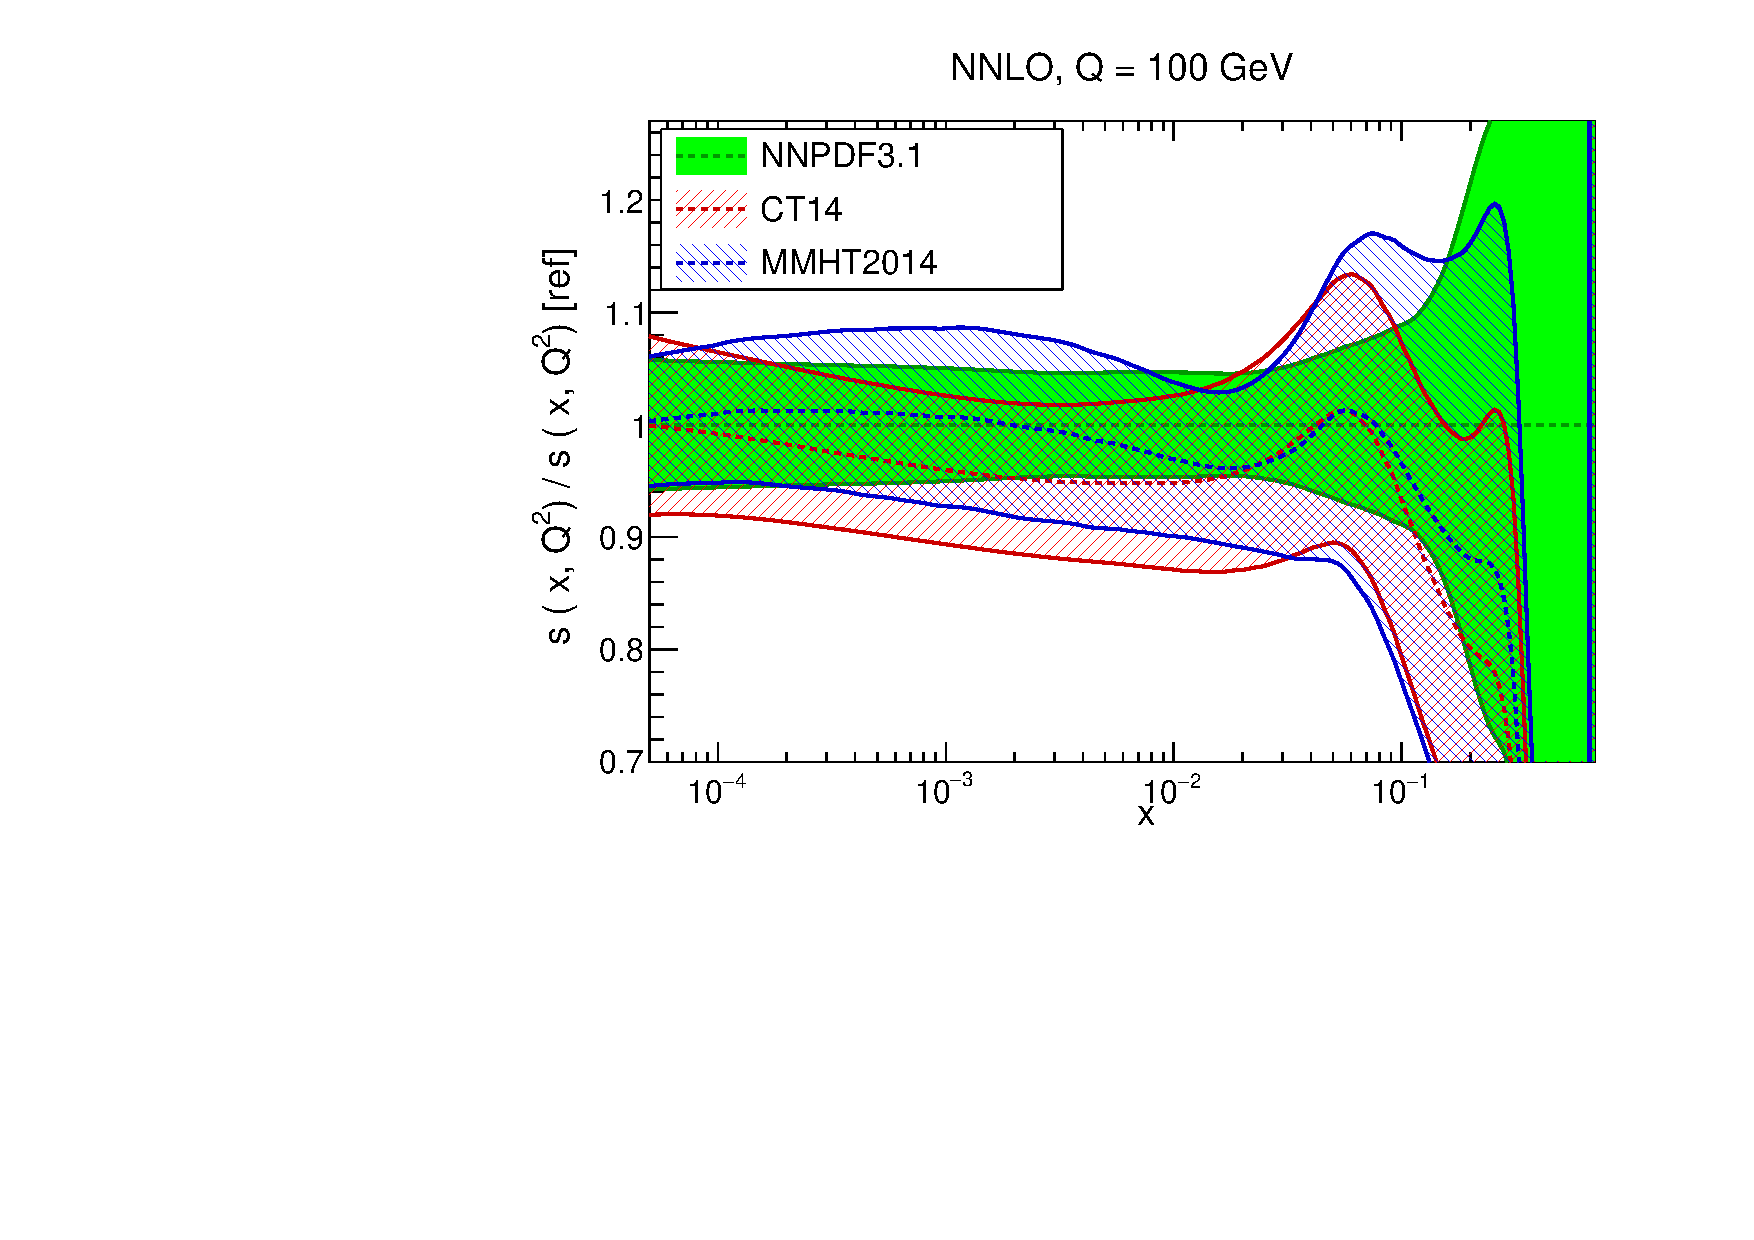
\includegraphics[scale=0.37]{plots/xs-31-nnlo-globalfits.pdf}
 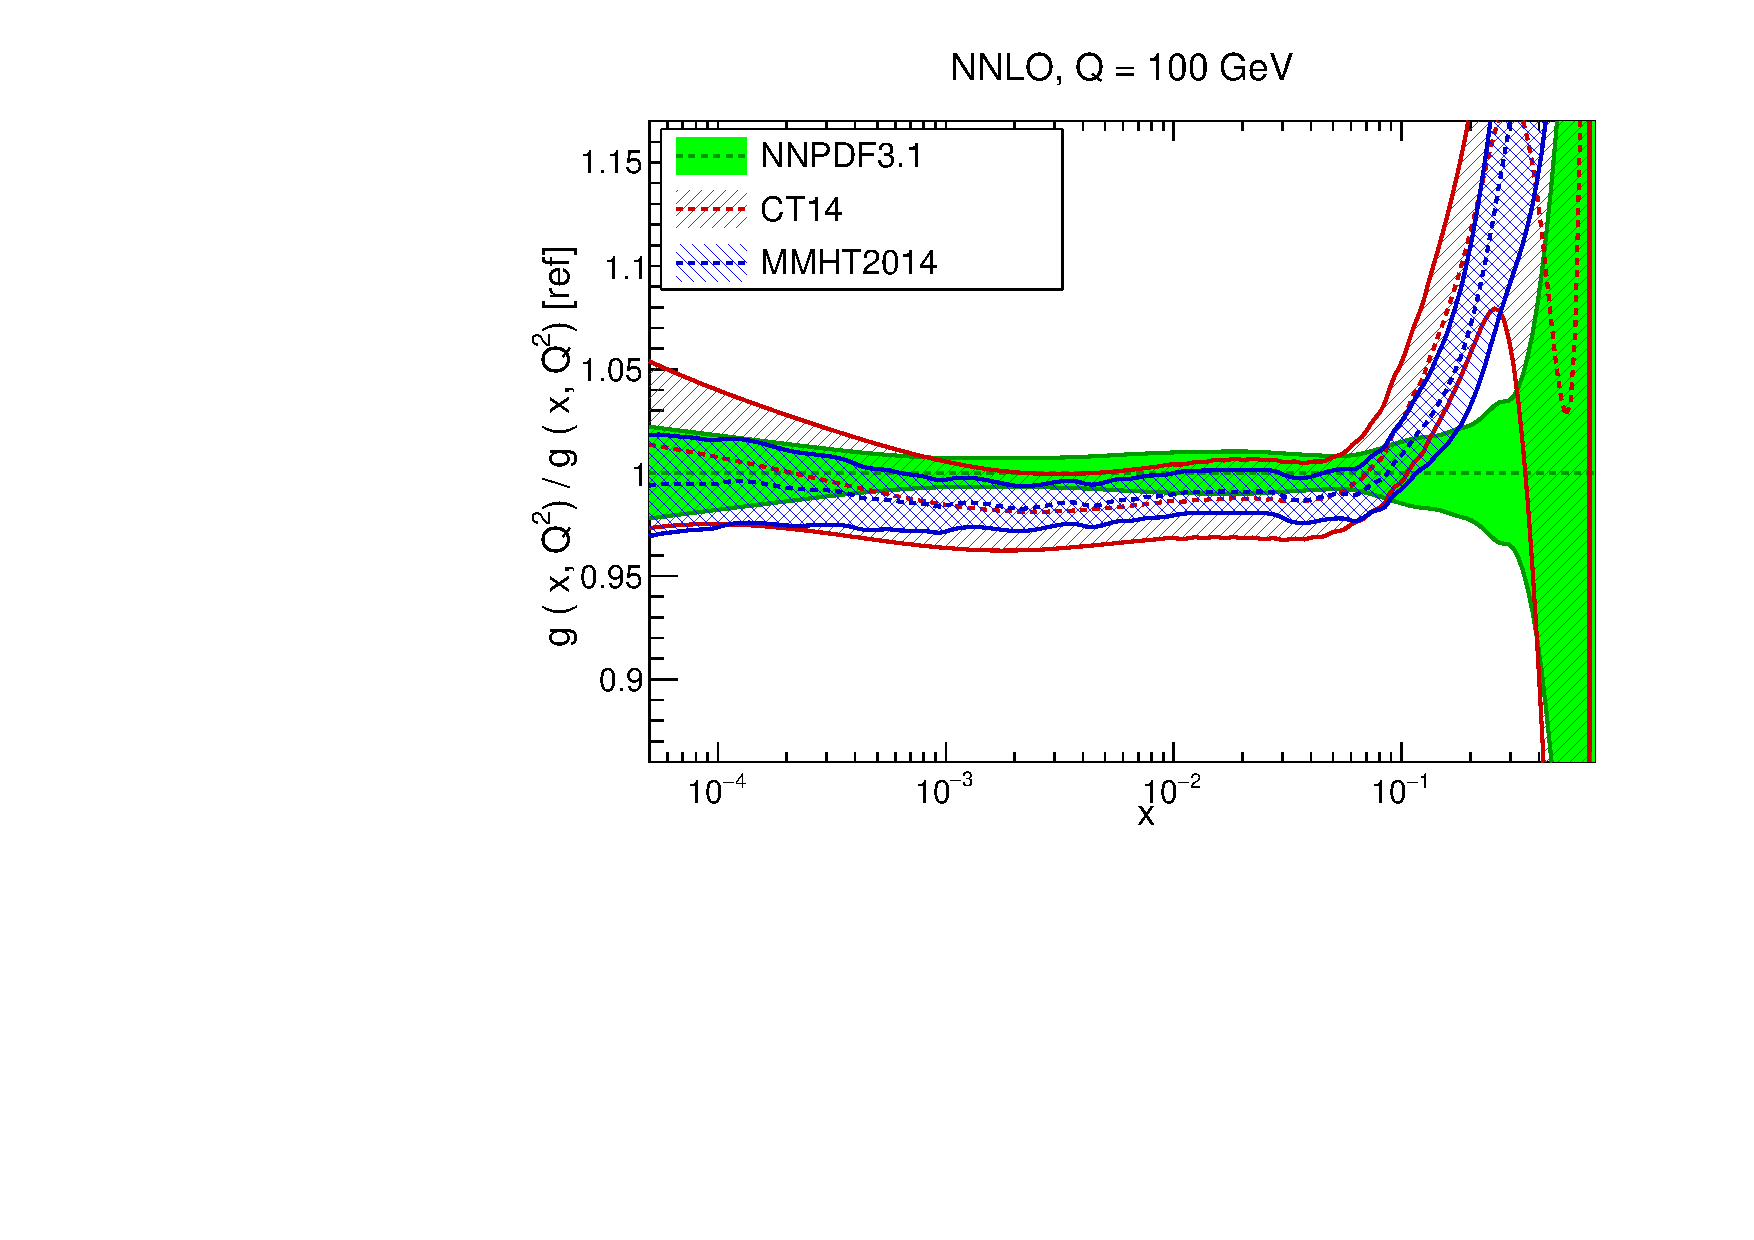
\includegraphics[scale=0.37]{plots/xg-31-nnlo-globalfits.pdf}\\
 \caption{\small Comparison between the CT14, MMHT2014
  and NNPDF3.1 NNLO PDF sets at $Q=100$ GeV, normalized
  to the central value of the latter.
  %
  From top to bottom and from left to right we show the
  $u$, $\bar{d}$ and $s$ quark PDFs as well as the gluon.
  %
  The error bands indicate the 1-$\sigma$ PDF uncertainties
  associated to each set.
  %
  These PDF comparison plots have been produced using the
  {\tt APFEL-Web} online plotting interface~\cite{Carrazza:2014gfa}.
    \label{fig:globalfits}
  }
\end{figure}
%-------------------------------------------------------------------------------

In addition to these latest versions of the global PDF fits,
there has recently been a significant development of techniques aiming
to construct combined PDF sets that are based on
a small number of Hessian eigenvectors or MC replicas and thus
are more efficient to use in lengthy higher-order
computations or Monte Carlo simulations.
%
In particular, the PDF4LHC15 PDF sets are based on the
combination of the CT14, MMHT14 and NNPDF3.1 NNLO PDF sets,
subsequently reduced to a small number of eigenvectors
(replicas) using the META-PDF~\cite{Gao:2013bia}
and MC2H~\cite{Carrazza:2015aoa}
(CMC~\cite{Carrazza:2015hva}) compression algorithms.
%
In this respect, Specialized Minimal PDF sets~\cite{Carrazza:2016htc}
(SM-PDFs) have also
been advocated, which
are tailored to specific physical processes and are based
on a minimal number of Hessian eigenvectors.
%
%The PDF4LHC15 sets provide a suitable representative for the expectations
%from the global QCD analysis point of view, and as such will be used
%in the benchmark comparisons of the next section.

The PDF4LHC15 NLO set~\cite{Butterworth:2015oua} is displayed in 
Fig.~\ref{fig:nnlopdfs} at $\mu^2=Q^2=4~{\rm GeV}^2$ and at
$\mu^2=Q^2=10^2~{\rm GeV}^2$.
%
Specifically, we show the $u_v=u-\bar{u}$ and $d_v=d-\bar{d}$ valence 
combinations, the $\bar{u}$, $\bar{d}$, $s$ and $c$ sea quark PDFs, 
and the gluon (divided by a factor 10).
%
The evolution between $Q^2=4$ GeV$^2$ to $Q^2=10^2$ GeV$^2$ is completely
determined by the solution of the DGLAP evolution equations.
%
The shape of the $u_v~(u^{-})$ and $d_v~(d^{-})$ valence quark combinations
reflects the constraints from the valence sum rules 
Eq.~(\ref{eq:valencesumrules}).
%
At small $x$, there is a rapid growth of the gluon and the sea quark PDFs, 
implying that the higher the collision center-of-mass energy $\sqrt{s}$, 
the more important gluon- and sea-quark-initiated processes become.
%
The bands in Fig.~\ref{fig:nnlopdfs} represent the 68\% CL PDF uncertainties.

%-------------------------------------------------------------------------------
\begin{figure}[!t]
\centering
  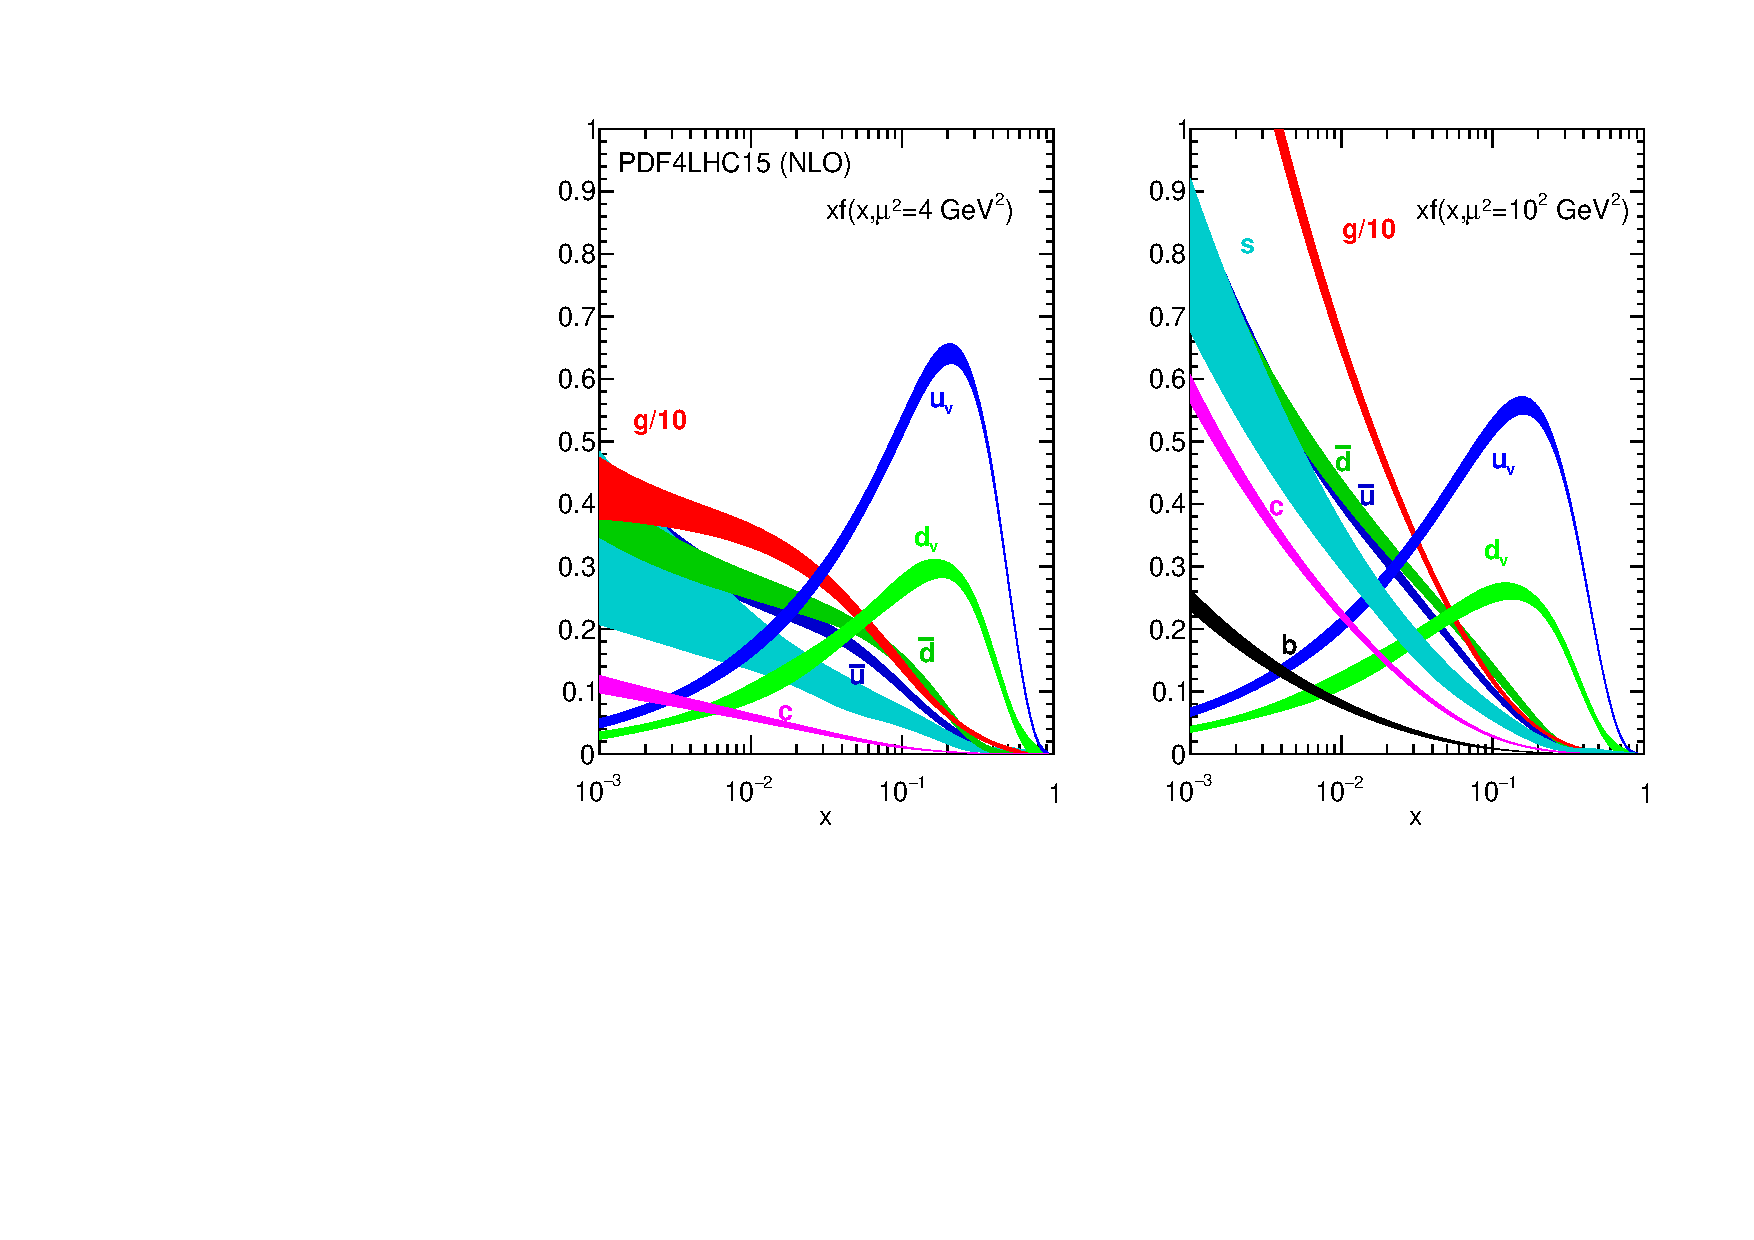
\includegraphics[scale=0.8]{plots/PDF4LHC15.pdf}\\
  \caption{\small The PDF4LHC15 NLO PDFs at a low scale
    $\mu^2=Q^2=4~{\rm GeV}^2$ (left plot) and at 
    $\mu^2=Q^2=10^2~{\rm GeV}^2$ (right plot) as a function of $x$.
    %
    We show the $u_v$ and $d_v$ valence combinations, the $\bar{u}$,
    $\bar{d}$, $s$ and $c$ sea quark PDFs, and the gluon (note that
    the latter is divided by a factor 10).
    \label{fig:nnlopdfs}
  }
\end{figure}
%-------------------------------------------------------------------------------

We strongly encourage the community to use the most recent versions
of global PDF fits when comparing with existing or new
lattice QCD calculations.
%
Comparing with deprecated sets, based on obsolete methodology
and in many cases experimental data that have been
superseded, should always be avoided.

\subsubsection{Polarized PDFs}
\label{sec:polPDFs}

\paragraph*{Theoretical features.}

The dependence on the momentum fraction $x$, fixed by nonperturbative QCD 
dynamics, should satisfy some theoretical constraints.
%
First, PDFs must lead to positive cross-sections.
At leading order (LO), this implies that polarized 
PDFs are bounded by their unpolarized counterparts\footnote{Beyond LO, more 
complicated relations hold~\cite{Altarelli:1998gn}; however they have little
effect on PDFs.}, $|\Delta f(x,\mu^2)|\leq f(x,\mu^2)$~\cite{Altarelli:1998gn}.
%
Second, PDFs must be integrable: this corresponds to the assumption 
that the nucleon matrix element of the axial current for each flavor is finite.
%
Third, SU(2) and SU(3) flavor symmetry, if assumed to be exact, imply that 
the zeroth moments of the nonsinglet $\mathcal{C}$-even PDF combinations,
$\Delta T_3=\Delta u^+ -\Delta d^+$ and 
$\Delta T_8 = \Delta u^+ +\Delta d^+ -2\Delta s^+$ 
(where $\Delta q^+=\Delta q+\Delta\bar{q}$, $q=u,d,s$), are respectively
related to the baryon octet $\beta$-decay constants, whose 
measured values are~\cite{Olive:2016xmw}
\begin{align}
 g_A  = a_3
 & =
 \int_0^1 dx \Delta T_3 (x,\mu^2)
 = \langle 1\rangle_{\Delta u^+} - \langle 1\rangle_{\Delta d^+}  = 1.2723 \pm 0.0023\,,
 \label{eq:a3}
 \\
 a_8
 & =
 \int_0^1 dx \Delta T_8 (x,\mu^2)
 = \langle 1 \rangle_{\Delta u^+} + \langle 1 \rangle_{\Delta d^+} -2\,\langle 1 \rangle_{\Delta s^+} 
 =0.585  \pm 0.025
 \,.
\label{eq:decayconst}
\end{align}
%
Fairly significant violations of SU(3) symmetry are advocated
in the literature (see {\it e.g.} Ref.~\cite{Cabibbo:2003cu} for a review). 
%
In this case, an uncertainty on the octet axial charge, larger by up to $30\%$ 
than its experimental value in Eq.~\eqref{eq:decayconst}, 
is found~\cite{FloresMendieta:1998ii}. 

\paragraph*{Experimental data.}
The bulk of the experimental information on polarized PDFs comes from 
neutral-current (photon exchange) inclusive and semi-inclusive deep-inelastic
scattering (DIS and SIDIS) with charged lepton beams and nuclear targets. 
%
As photon scattering does not distinguish quarks and antiquarks, inclusive DIS 
data constrain only the total quark combinations $\Delta q^+$, 
while SIDIS data with identified pions or kaons in the final state 
constrain individual quark and antiquark flavors. 
%
In principle, both DIS and SIDIS are also sensitive to the gluon 
distribution $\Delta g$, as it directly enters the factorized expressions of
the corresponding structure functions beyond LO, and indirectly via DGLAP 
evolution.
%
In practice, the constraining power of DIS and SIDIS data on $\Delta g$ is 
rather weak because the $Q^2$ range covered by the data is limited,
especially if one restricts to the kinematic region not affected by
power-suppressed corrections and very precise data from JLab are therefore
excluded. 

Note that, in the case of SIDIS, a reliable knowledge of fragmentation 
functions (FFs) is required in the factorized expressions of the 
corresponding observables. 
%
Since FFs are nonperturbative objects on the same footing as PDFs, they are 
an additional source of uncertainty in PDF determinations, if not a bias.
%
A significant experimental and theoretical effort has been
invested in improving the independent determination of 
FFs~\cite{deFlorian:2014xna,deFlorian:2017lwf,
Hirai:2016loo,Sato:2016wqj,Bertone:2017tyb} and most recently in simultaneously 
fitting both PDFs and FFs~\cite{Ethier:2017zbq}.

Besides DIS and SIDIS fixed-target data, a significant amount of data from
longitudinally polarized proton-proton collisions at the Relativistic 
Heavy Ion Collider (RHIC) has become available recently (see {\it e.g.} 
Ref.~\cite{Aschenauer:2015eha} for an overview), although in a limited range 
of momentum fractions, $0.05\lesssim x \lesssim 0.4$.
%
On the one hand, longitudinal (parity-violating) single-spin and 
(parity-conserving) double-spin asymmetries for $W^\pm$ boson production are 
sensitive to the flavor decomposition of polarized quark and antiquark 
distributions, because of the chiral nature of the weak 
interaction~\cite{Bourrely:1993dd}. 
%
On the other hand, double-spin asymmetries for jet, di-jet and $\pi^0$ 
production are directly sensitive to the gluon polarization in 
the proton, because of the dominance of gluon-gluon and quark-gluon initiated 
subprocesses in the kinematic range accessed by RHIC~\cite{Bourrely:1990pz}.

The kinematic coverage of the data that can be used to constrain polarized 
PDFs is displayed in Fig.~\ref{fig:kinEIC}.
%
A comparison with Fig.~\ref{fig:kinplot-report} makes it apparent that the
quantity of data points, their kinematic coverage and the variety of 
available hard-scattering processes are presently much more limited in the 
polarized case than in the unpolarized case.
%
Therefore, polarized PDFs can currently be determined with much less 
precision than their unpolarized counterparts and only over an $x$-range limited
to $x\gtrsim 0.005$.
%
The kinematic coverage is expected to be significantly extended in the future,
with DIS and SIDIS data from JLab-12~\cite{Dudek:2012vr} and a polarized 
high-energy Electron-Ion Collider (EIC)~\cite{Accardi:2012qut}.
%
Such an extended kinematic coverage is also displayed in Fig.~\ref{fig:kinEIC},
where it is denoted as eRHIC.

%-------------------------------------------------------------------------------
\begin{figure}[!t]
\centering
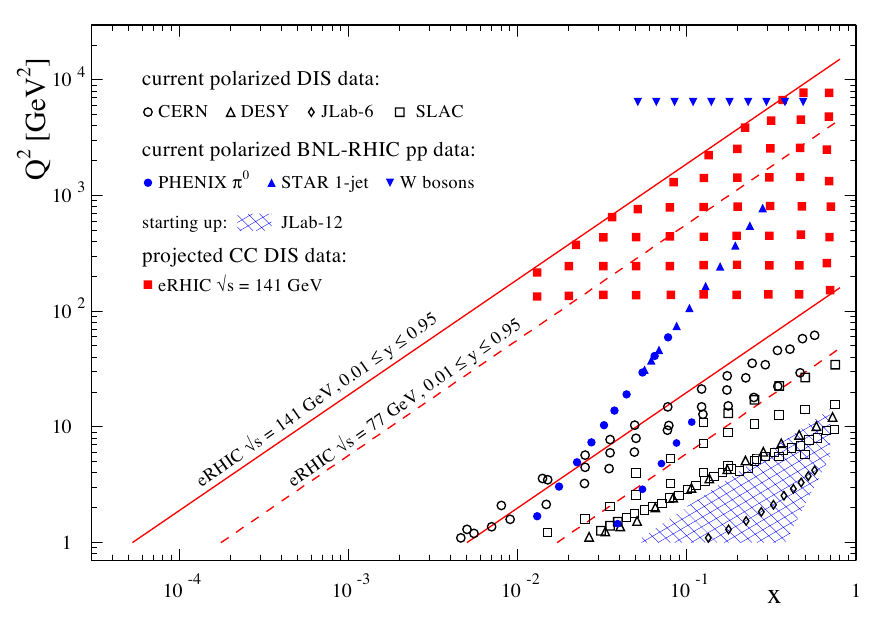
\includegraphics[width=0.9\textwidth]{plots/kinEIC}\\
\caption{\small Representative kinematic coverage, in the $(x,Q^2)$ plane,
of the (neutral current) DIS, SIDIS and proton-proton hard-scattering 
measurements that are used as input in a global polarized PDF fit.
%
The extended kinematic coverage achieved by 
JLab-12~\cite{Dudek:2012vr} and by an EIC~\cite{Accardi:2012qut}
(including projected charged-current (CC) DIS data and denoted as eRHIC) 
is also shown.
%
Figure taken from Ref.~\cite{Aschenauer:2014cki}.}
\label{fig:kinEIC}
\end{figure}
%-------------------------------------------------------------------------------

A representative illustration of polarized PDFs obtained from a global
QCD analysis, namely NNDPFpol1.1~\cite{Nocera:2014gqa}, is provided in Fig.~\ref{fig:qPDFpol}.
%
The format is the same as for the unpolarized case, Fig.~\ref{fig:nnlopdfs},
in order to ease any comparison between the two.
%
In particular, note the suppression of all polarized PDFs at small values of 
$x$, including polarized sea quark PDFs, with respect to their unpolarized 
counterparts.

%-------------------------------------------------------------------------------
\begin{figure}[!t]
\centering
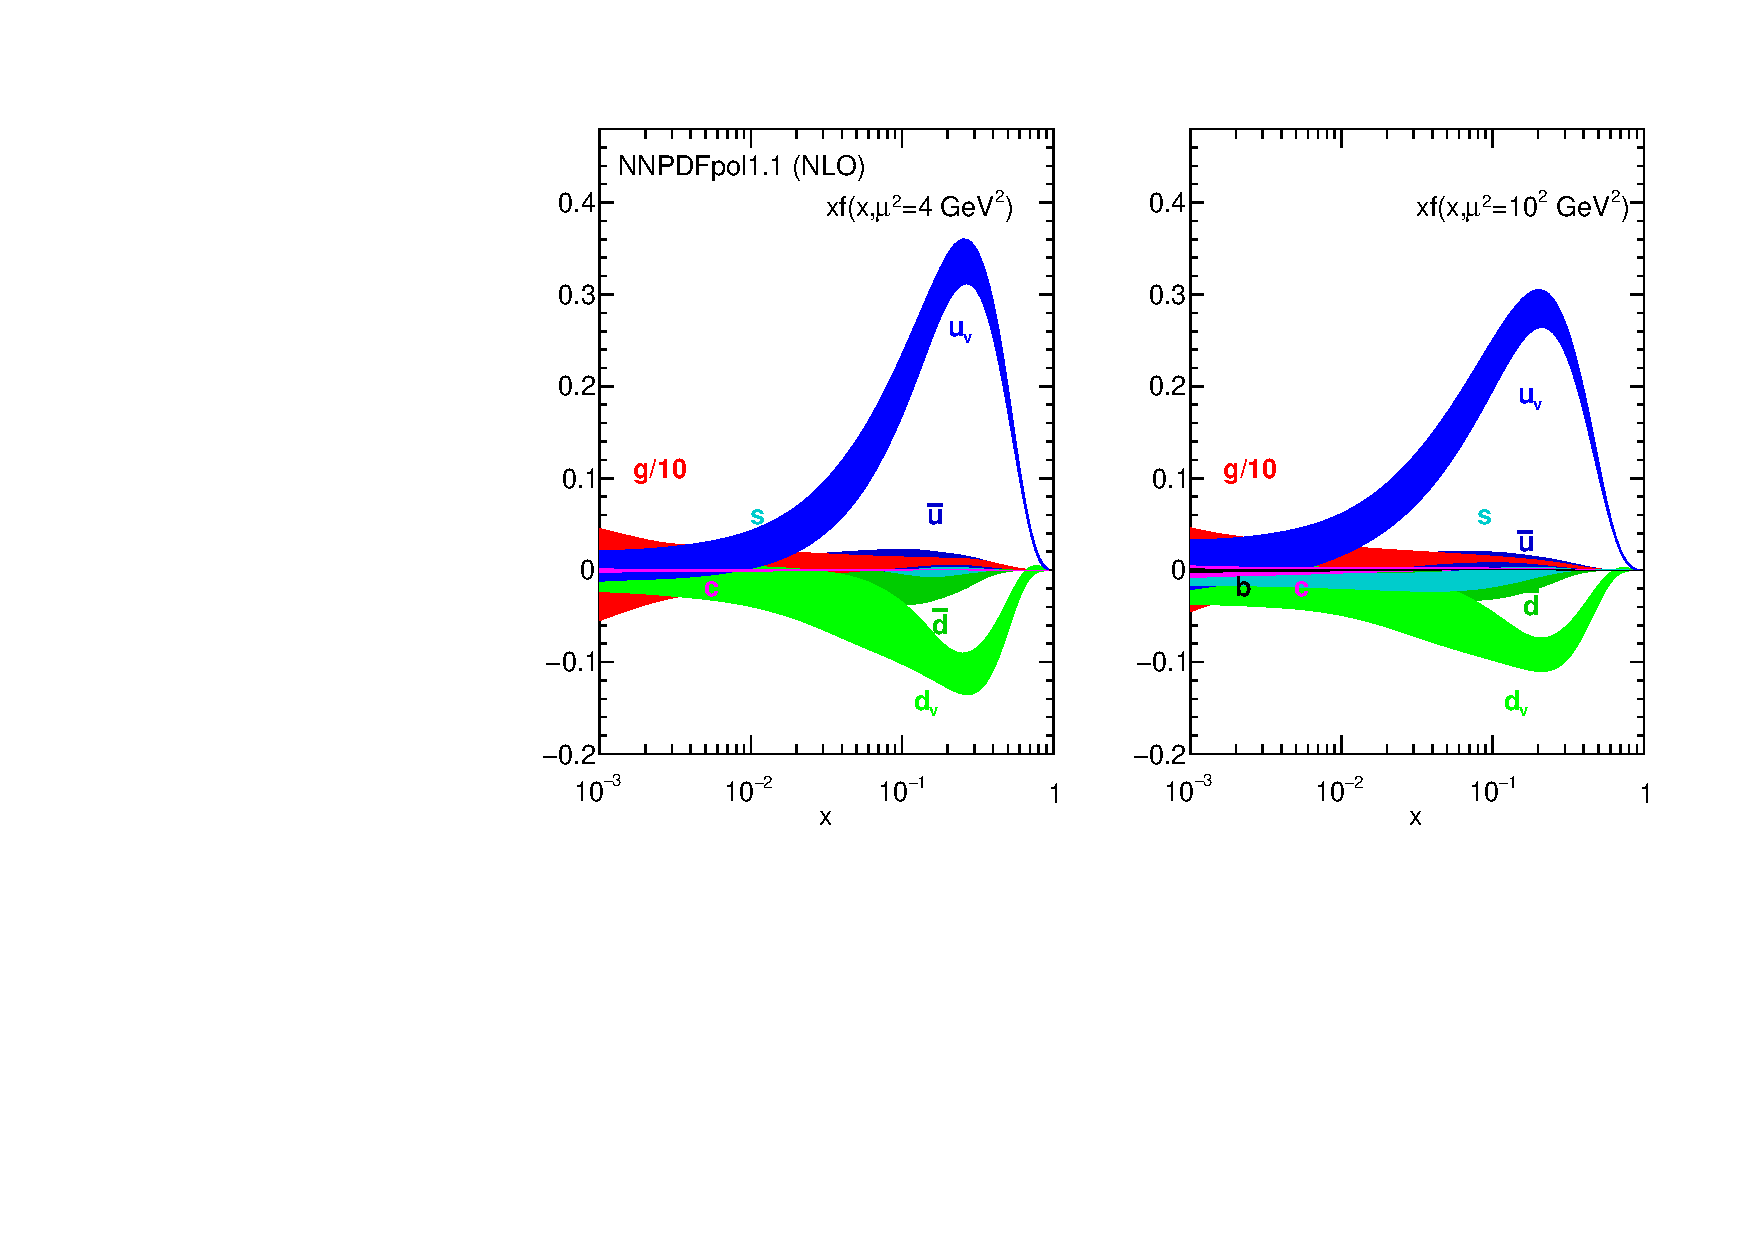
\includegraphics[scale=0.8]{plots/NNPDFpol11}\\
\caption{\small Same as Fig.~\ref{fig:nnlopdfs}, 
but for the polarized NNPDFpol1.1 NLO PDFs~\cite{Nocera:2014gqa}.}
\label{fig:qPDFpol}
\end{figure}
%-------------------------------------------------------------------------------

\paragraph{State-of-the-art global PDF fits.}

Several modern determinations of polarized PDFs of the proton (up to 
NLO\footnote{A NNLO QCD analysis of polarized PDFs based on inclusive DIS
data only was performed in Refs.~\cite{Shahri:2016uzl,Khanpour:2017cha}.
Inclusive DIS is the only polarized process for which coefficient functions
are known up to NNLO (all others are known up to NLO).} 
and mostly in the $\overline{\rm MS}$ factorization scheme) are available in 
the literature~\cite{Nocera:2014gqa,Nocera:2016xhb,deFlorian:2014yva,deFlorian:2008mr,deFlorian:2009vb,Sato:2016tuz,Leader:2010rb,Blumlein:2010rn,Bourrely:2014uha,Hirai:2008aj}. 
%
A key goal of these is to unveil the size (and uncertainty) of
$\Delta\Sigma$ and  $\Delta G$ in Eq.~\eqref{eq:moments}. 
%
The various determinations differ among each other in the data sets included 
in the analysis, in some details of the QCD analysis (like the treatment of 
higher-twist corrections) and in the procedure used to determine PDFs from the 
data (for details, see {\it e.g.} Chap.~3 in Refs.~\cite{Nocera:2014vla} 
and~\cite{Nocera:2016xhb,Jimenez-Delgado:2013sma}). 
%
The NNDPF procedure and the standard (adopted by DSSV) have 
already been outlined in Sec.~\ref{sec:genframework}. 
%
We note that DSSV has developed a method based on Mellin moments of the PDFs 
in order to efficiently incorporate NLO computations
of proton-proton cross-sections in the fitting procedure. 
%
The JAM collaboration has implemented a new approach called 
iterative Monte Carlo procedure~\cite{Sato:2016tuz,Ethier:2017zbq}
in their analyses.

The most recent analyses of polarized PDFs are DSSV14~\cite{deFlorian:2014yva}
and NNPDFpol1.1~\cite{Nocera:2014gqa}.
%
Motivated by the interest in assessing the impact of RHIC proton-proton 
data, they upgrade the corresponding previous analyses, 
DSSV08~\cite{deFlorian:2008mr,deFlorian:2009vb} and 
NNPDFpol1.0~\cite{Ball:2013lla}, with data respectively on double-spin 
asymmetries for inclusive jet production~\cite{Adamczyk:2014ozi} 
and $\pi^0$ production~\cite{Adare:2014hsq}\footnote{Preliminary RHIC results 
included in Ref.~\cite{deFlorian:2008mr} were replaced in
Ref.~\cite{deFlorian:2014yva} with final results.}, 
and on double-spin asymmetries for high-$p_T$ inclusive jet 
production~\cite{Adamczyk:2014ozi,Adamczyk:2012qj,Adare:2010cc} and single-spin
asymmetries for $W^\pm$ production~\cite{Adamczyk:2014xyw}.
%
The new data have been included in NNPDFpol1.1 
by means of Bayesian reweighting~\cite{Ball:2010gb},
and in DSSV14 by means of a full refit.  

Overall, both the DSSV14 and NNPDFpol1.1 PDF determinations are 
state-of-the-art in the inclusion of the available experimental information. 
%
The data sets in the two analyses differ between each other only in
fixed-target SIDIS and RHIC $\pi^0$ production measurements, included in 
DSSV14, but not in NNPDFpol1.1. 
%
The information brought in by these data is complementary to that provided by 
RHIC $W^\pm$ production and inclusive jet production data respectively,
although fraught with larger theoretical uncertainties related to fragmentation.

%------------------------------------------------------------------------------
\begin{figure}[!t]
\centering
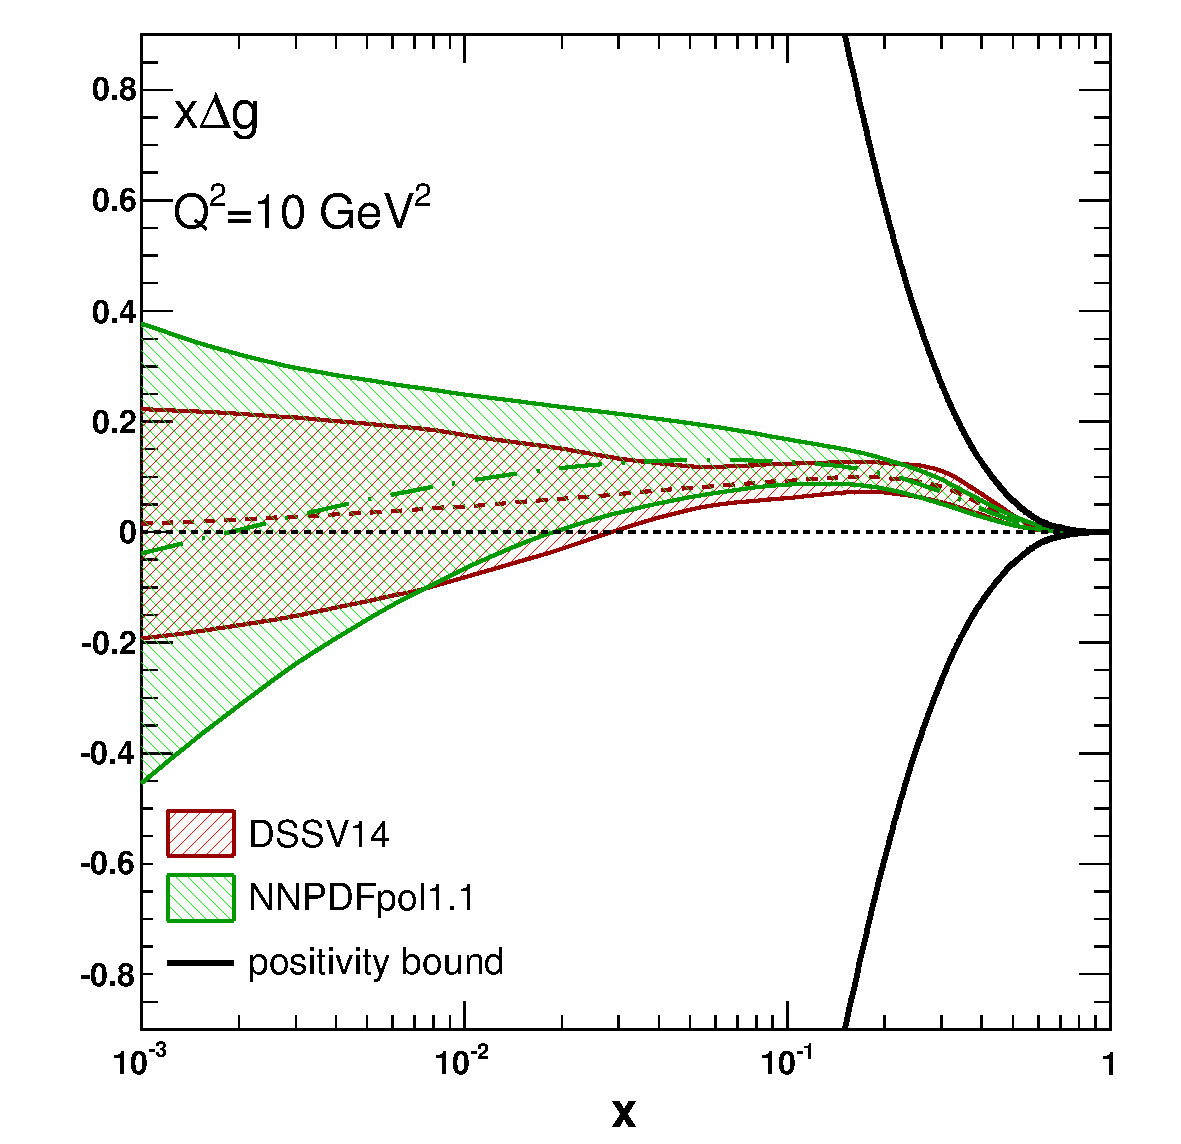
\includegraphics[scale=0.33,clip=true,trim= 0 -1.3cm 0 0]{plots/gluoncomp}
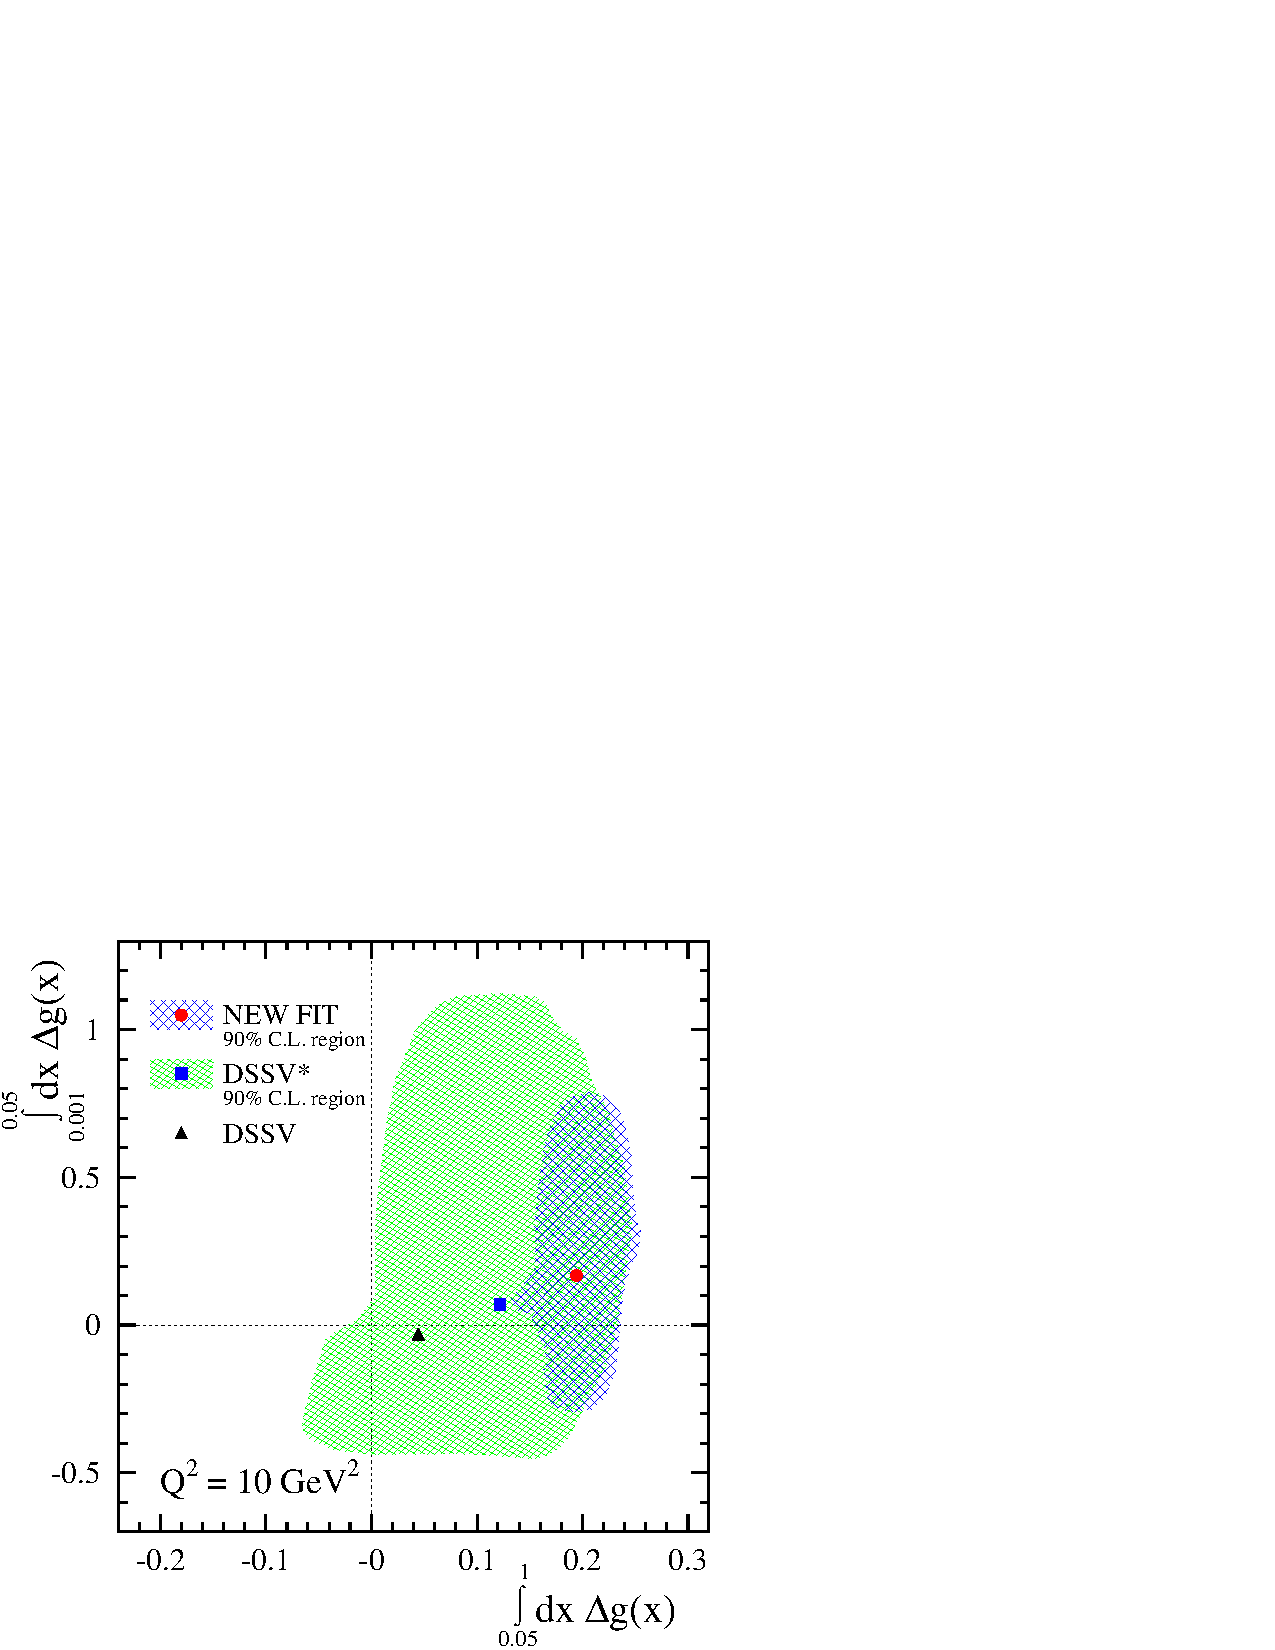
\includegraphics[scale=0.555,clip=true,trim=0 0 7cm 15cm]{plots/correlation_getot.pdf}\\
\caption{\small (Left) The polarized gluon momentum distribution  
$x\Delta g$ from the DSSV14 (with $90\%$ C.L. uncertainty band)
and NNPDFpol1.1 PDF sets at $Q^2=10$ GeV$^2$. The NNPDF3.1 positivity
bound is also shown.
(Right) $90\%$ C.L.\ areas in the plane spanned by the truncated moments of
$\Delta g$ computed for $0.05\leq x\leq 1$ and $0.001\leq x\leq 0.05$ at $Q^2=10\,\mathrm{GeV}^2$~\cite{deFlorian:2014yva}.}
\label{fig:RHICpdfs}
\end{figure}
%------------------------------------------------------------------------------

The effect of RHIC data on the polarized PDFs of the proton is twofold:
\begin{itemize}

\item The 2009 STAR and PHENIX data sets on jet and $\pi^0$ 
production~\cite{Adamczyk:2014ozi,Adare:2014hsq}, included in DSSV14
and NNPDFpol1.1, provide the first evidence
of a sizable positive gluon polarization in the proton. 
%
A comparison of the gluon PDF in the two PDF sets is displayed in 
Fig.~\ref{fig:RHICpdfs} (left panel). 
%
Comparable results, both central values and uncertainties, are found in the 
$x$ region covered by RHIC data. 
%
The agreement between the two analyses is optimal in the
range $0.08\leq x \leq 0.2$, where the dominant experimental information comes
from jet data; a slightly smaller central value is found in the DSSV14 
analysis, in comparison to NNPDFpol1.1, in the range 
$0.05\leq x \leq 0.08$, where the dominant experimental information comes from 
$\pi^0$ production data. 
%
Indeed, these are included in DSSV14 but are not in NNPDFpol1.1. 
%
Nevertheless, best fits lie well within each other's error
bands, though NNPDFpol1.1 uncertainties tend to be larger than DSSV14
uncertainties outside the region covered by RHIC data.
%
Very consistent values of the zeroth moment of $\Delta g$, 
Eq.~\eqref{eq:moments}, truncated over the interval $0.05\leq x \leq 1$, are 
found: at $Q^2=10$ GeV$^2$, this is $0.20^{+0.06}_{-0.07}$ for 
DSSV14~\cite{deFlorian:2014yva}, and $0.23\pm 0.06$ for 
NNPDFpol1.1~\cite{Nocera:2014gqa}. The right plot in Fig.~\ref{fig:RHICpdfs} 
shows the corresponding DSSV14 result as an example; the impact of the RHIC
data is clearly visible. 

\item The 2012 STAR data sets on $W$ production~\cite{Adamczyk:2014xyw}, 
included in NNPDFpol1.1, provide evidence of a positive 
$\Delta\bar{u}$ distribution 
and a negative $\Delta\bar{d}$ distribution, with 
$|\Delta\bar{d}|>|\Delta\bar{u}|$~\cite{Nocera:2014gqa},
as shown in Fig.~\ref{fig:RHICpdfs1}.
% 
The size of the flavor symmetry breaking for polarized sea quarks is 
quantified by the asymmetry $\Delta\bar{u}-\Delta\bar{d}$, which,
in the NNPDFpol1.1 analysis, turn out to be roughly as large as its 
unpolarized counterpart (in absolute value)~\cite{Ball:2017nwa}, 
though much more uncertain~\cite{Nocera:2014rea}. 
%
Even within this uncertainty, polarized and unpolarized light sea quark 
asymmetries show opposite signs, with the polarized one being clearly positive. 
% 
This trend is also found from analysis of the polarized SIDIS data, 
as revealed by the DSSV08 parton set. 
%
This result may discriminate among various models of nucleon structure, 
see~\cite{Nocera:2014rea} and references therein. 
%Fig.~\ref{fig:RHICpdfs1}: 
%specifically, some meson-cloud (MC) models are disfavored, while a more 
%accurate experimental information is needed to establish whether 
%chiral quark-soliton (CQS), Pauli-blocking (PB) or statistical (ST)
%models are preferred (all these models are described in~\cite{Chang:2014jba}).

\end{itemize}

%------------------------------------------------------------------------------
%\begin{figure}[!h]
%\centering
%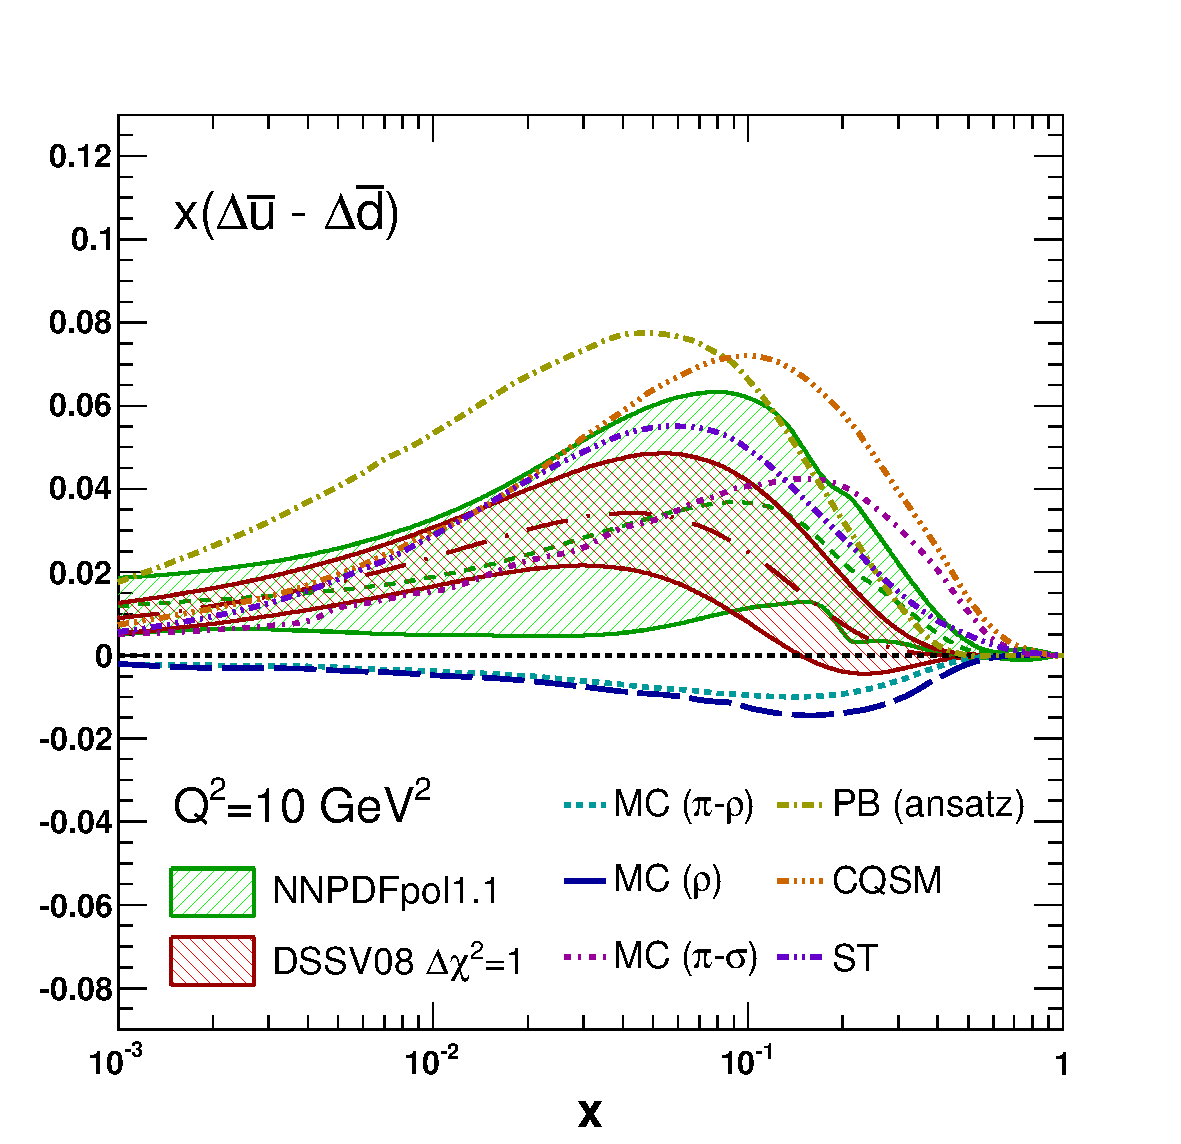
\includegraphics[scale=0.35]{plots/asysea_2}\\
%\caption{\small The polarized light sea quark asymmetry 
%$x(\Delta\bar{u}-\Delta\bar{d})$ from the NNPDFpol1.1 and 
%DSSV08 PDF sets at $Q^2=10$ GeV$^2$, compared to expectations from 
%various models of nucleon structure~\cite{Chang:2014jba}.}
%\label{fig:RHICpdfs1}
%\end{figure}
%------------------------------------------------------------------------------

\paragraph{Open issues.}

Despite the achievements described above, the polarized PDFs presently cannot 
be determined in a global QCD analysis with the same accuracy as their 
unpolarized counterparts.
%
The experimental data are confined to a relatively narrow range of 
$x$ and $Q^2$.
%
As a consequence, the size of the contributions of quarks, antiquarks and 
gluons to the nucleon spin, as quantified by their zeroth moments, 
Eq.~\eqref{eq:moments}, are still affected by large uncertainties. 
%
These come predominantly from the extrapolation into the small-$x$ region 
($x\lesssim 10^{-3}$). 
%
Here potential modifications in the PDF shape induced by small-$x$ 
evolution~\cite{Bartels:1995iu,Bartels:1996wc,Kovchegov:2015pbl,
Kovchegov:2016weo,Kovchegov:2016zex,Kovchegov:2017jxc,Kovchegov:2017lsr} 
could arise, which presently cannot be tested.
%
Significant uncertainties also affect the PDFs in the large-$x$ 
{\it valence} region ($x\gtrsim 0.7$). 
%
This regime is less relevant for the determination of the PDF moments, but it 
is important for comparisons to nonperturbative models of nucleon structure, 
especially in terms of ratios of light-quark polarized to unpolarized PDFs 
(for a comparison between large-$x$ PDFs 
and model predictions, see Ref.~\cite{Nocera:2014uea}).
%
Finally, the small lever arm of the data in $Q^2$ is a serious limiting factor 
in the determination of $\Delta g$ via evolution, unless the data at low $Q^2$
and large $x$ are included in the fit and carefully analyzed.
%
This requires an appropriate treatment of power-suppressed corrections and 
possibly a minimization methodology which can iteratively focus on a region 
in parameter space where constraints are not too strong, as done in the 
JAM15 analysis~\cite{Sato:2016tuz}. 

The determination of the total polarized strange distribution $\Delta s^+$ is 
also particularly delicate.
%
Inclusive DIS data, together with nonsinglet axial couplings, 
Eq.~\eqref{eq:decayconst}, and kaon SIDIS data provide the sole available 
constraint on $\Delta s^+$.
%
A sizable negative $\Delta s^+$ is found 
consistently in all analyses based on inclusive DIS data only, as a result 
of the constraint from hyperon decays that is usually adopted. 
%
However, the shape of $\Delta s^+$ may change significantly in analyses that also include
SIDIS data. Typically SIDIS data lead to a trend for $\Delta s^+$ to be
small or even slightly positive in the medium $x$-range, although this depends 
also on the set of kaon FFs used to compute
the corresponding observables~\cite{Leader:2011tm}.  
%
The recent study in Ref.~\cite{Ethier:2017zbq} sheds some light on this issue
by performing a simultaneous determination of polarized PDFs and unpolarized 
FFs using DIS, SIDIS and single-inclusive annihilation data.
%
In order to avoid biasing the determination of $\Delta s^+$ by 
assumptions on SU(3) symmetry, the octet axial charge in 
Eq.~\eqref{eq:decayconst} has been allowed to be determined by the data alone.
%
As a consequence, a slightly positive $\Delta s^+$ distribution, but
compatible with the negative result found from inclusive DIS within its 
large uncertainties, has been obtained.
% 
An octet axial charge about $20\%$ smaller than its quoted experimental value, 
Eq.~\eqref{eq:decayconst}, appears to be preferred by the data.
%
This change is opposite in sign to that in~\cite{FloresMendieta:1998ii}.
%
However, we stress that the determination of $\Delta s^+$ from SIDIS data 
also relies on good knowledge of the {\it un}polarized strange distribution. 
%
Furthermore, unpolarized SIDIS data themselves set constraints on 
FFs and ultimately would need to be included as well
to obtain a reliable picture. 
%
In any case, further higher precision kaon SIDIS data will be needed 
to reduce the uncertainty on $\Delta s^+$ and further test the degree of 
SU(3) breaking. 

Ongoing and future experimental campaigns at current facilities are
expected to provide additional experimental information
useful to clarify some of the issues outlined above (for an 
assessment of the impact of very recent/forthcoming data, see {\it e.g.}
Refs.~\cite{Aschenauer:2015eha,Aschenauer:2015ata,Nocera:2015vva,
Nocera:2017wep}).
%
However, a future high-energy, polarized EIC~\cite{Accardi:2012qut} will 
likely be the only facility to be able to address all of the above issues 
with the highest precision. 
% 
The extension of the kinematic reach down to $x\sim 10^{-4}$ and up to
$Q^2=10^4$ GeV$^2$ will allow for an accurate determination of $\Delta g$
via evolution in DIS/SIDIS, of $\Delta\bar{u}$ and 
$\Delta\bar{d}$ via inclusive DIS at high $Q^2$ mediated by electroweak bosons,
and of $\Delta s$ via kaon-tagged SIDIS. 
%
The potential impact of the longitudinally polarized program at an EIC
has been quantitatively assessed in several dedicated 
studies~\cite{Aschenauer:2012ve,Ball:2013tyh,Aschenauer:2013iia,
Aschenauer:2015ata}.

